%--------sigalternate----------
\documentclass{sig-alternate}
%--------/sigalternate----------

%\documentclass[letterpaper,twocolumn,10pt]{article}
\usepackage{endnotes,multirow}
\usepackage{refstyle,amsmath,chngcntr}
\usepackage{epsfig,subfigure,framed}
%\usepackage{multicol,tabularx}
\usepackage{textcomp} % for tilde
\usepackage{paralist} % for in-paragraph lists
\usepackage{graphicx}
%\usepackage{epstopdf}
%\epstopdfsetup{update} % only regenerate pdf files when eps file is newer

\iffalse
\usepackage[]{hyperref}
\hypersetup{
    pdftitle={Behave or Be Watched: Debugging With Behavioral Watchpoints},
    pdfauthor={Akshay Kumar, Peter Goodman, Angela Demke Brown, Ashvin Goel},
    pdfkeywords={watchpoints,debugging,binary translation,dbt,instrumentation},
    bookmarksnumbered=true,     
    bookmarksopen=true,         
    bookmarksopenlevel=1,       
    colorlinks=true,
    allcolors=black,
    pdfstartview=Fit,           
    pdfpagemode=UseOutlines,    % this is the option you were lookin for
    pdfpagelayout=TwoPageRight
}
\fi

% Used for code snippets
\usepackage{listings,courier}

% Used for changing the spacing after the title, sections, and subsections.
%--------sigalternate----------\newcommand{\subparagraph}{}
%--------sigalternate----------\usepackage{titlesec}

% Make text in figure captions small
\usepackage{caption3} % load caption package kernel first
%\DeclareCaptionOption{parskip}[]{} % disable "parskip" caption option
\usepackage{caption}
\DeclareCaptionType{copyrightbox}

% Make sure that figure numbers are continuous through the document
\counterwithout{figure}{section}
\counterwithout{figure}{subsection}

% Settings on code listings.
\lstset{language=C,
		xleftmargin=0pt,
		xrightmargin=0pt,
		framexbottommargin=0pt,
        framextopmargin=0pt,
        framesep=0pt}

% Modify spacing before/after title, sections, and subsections.
%\setlength{\droptitle}{-3em}  %--------sigalternate----------
%\posttitle{\par\end{center}\vspace{-1.5em}} %--------sigalternate----------
\newcommand{\Sref}[1]{Section~\ref{#1}} 

%--------sigalternate----------\titlespacing\section{0pt}{5pt plus 4pt minus 2pt}{5pt plus 2pt minus 2pt}        
%--------sigalternate----------\titlespacing\subsection{0pt}{5pt plus 4pt minus 2pt}{5pt plus 2pt minus 2pt}   

% Compressed enumerations
\newenvironment{enumerate*}%
  {\begin{enumerate}%
    \setlength{\itemsep}{2pt}%
    \setlength{\parskip}{0pt}}%
  {\end{enumerate}}

% Compressed bibliography
%\let\ORIGbibliography\bibliography
%\renewcommand{\bibliography}[1]{{\footnotesize \ORIGbibliography{#1}}}

% Add a horizontal rule above captions, and make captions closer to their figures
\DeclareCaptionFormat{ruled_caption}{#1#2#3\hrulefill}
\captionsetup[figure]{format=ruled_caption}
%\let\ORIGcaption\caption
%\renewcommand{\caption}[2][\compressedcaption]{%
%\def\compressedcaption{#2}%
%    \vspace{-12pt}%
%    \ORIGcaption[#1]{#2}%
%    \vspace{-12pt}}

% Decrease spacing before \paragraphs
%--------sigalternate----------\titlespacing{\paragraph}{%
%--------sigalternate----------  0pt}{%              left margin
%--------sigalternate----------  0.25\baselineskip}{% space before (vertical)
%--------sigalternate----------  1em}%               space after (horizontal)

% Prevent footnotes from spanning multiple pages
\interfootnotelinepenalty=10000

% For leaving some comments in the draft.
\newcommand{\comment}[1]{}

%\begin{document}
%--------sigalternate----------
\begin{document}
%
% --- Author Metadata here ---
\conferenceinfo{HotDep - Workshop on Hot Topics in Dependable Systems}{November 3, 2013, Nemacolin Woodlands Resort (PA), USA}
\CopyrightYear{2013} % Allows default copyright year (20XX) to be over-ridden - IF NEED BE.
\crdata{978-1-4503-2457-1}  % Allows default copyright data (0-89791-88-6/97/05) to be over-ridden - IF NEED BE.
% --- End of Author Metadata ---
%--------/sigalternate----------

%don't want date printed
\date{}

\conferenceinfo{\\\\HotDep}{'13, November 03-06, 2013, Farmington, PA, USA}

\CopyrightYear{2013} % Allows default copyright year (20XX) to be over-ridden - IF NEED BE.
\crdata{Copyright is held by the owner/author(s). Publication rights licensed to ACM.  ACM 978-1-4503-2457-1/13/11 ...\$15.00. \\http://dx.doi.org/10.1145/2524224.2524234}  % Allows default copyright data (0-89791-88-6/97/05) to be over-ridden - IF NEED BE.

%make title bold and 14 pt font (Latex default is non-bold, 16 pt)
\title{\Large \bf Behave or Be Watched: Debugging with Behavioral Watchpoints}

%for single author (just remove % characters)
%\author{
%{\rm Akshay Kumar} \hspace{1.5em} {\rm Peter Goodman} \hspace{1.5em}  {\rm Angela Demke Brown} \hspace{1.5em} {\rm Ashvin Goel}\\
%University of Toronto
%} % end author


\numberofauthors{4} %  in this sample file, there are a *total*
% of EIGHT authors. SIX appear on the 'first-page' (for formatting
% reasons) and the remaining two appear in the \additionalauthors section.
%
\author{
% You can go ahead and credit any number of authors here,
% e.g. one 'row of three' or two rows (consisting of one row of three
% and a second row of one, two or three).
%
% The command \alignauthor (no curly braces needed) should
% precede each author name, affiliation/snail-mail address and
% e-mail address. Additionally, tag each line of
% affiliation/address with \affaddr, and tag the
% e-mail address with \email.
%
% 1st. author
\alignauthor
Akshay Kumar\\
       \email{akshay@eecg.toronto.edu}
% 2nd. author
\alignauthor
Peter Goodman\\
       \email{pag@cs.toronto.edu}
\and
% 3rd. author
\alignauthor
Ashvin Goel\\
       \email{asvhin@eecg.toronto.edu}
% 4th. author
\alignauthor
Angela Demke Brown\\
       \email{demke@cs.toronto.edu}
}


\maketitle
%\subsection*{Abstract}
\begin{abstract}
Finding, understanding, and fixing bugs in an operating system is challenging. Dynamic binary translation (DBT) systems provide a powerful facility for building program analysis and debugging tools. However, DBT abstractions are too low-level and provide limited contextual information for instrumentation tools.

We introduce \emph{behavioral watchpoints}, a new software-based watchpoint framework that simplifies the implementation of DBT-based program analysis and debugging tools. Behavioral watchpoints extend the traditional approach of using a DBT system by providing context-specific information at the instruction level and specializing instrumentation to individual data structures. We describe four applications developed using our watchpoint framework: detecting buffer overflows, detecting read-before-write and memory freeing bugs, detecting memory leaks and enforcing fine-grained memory access policies. We implemented behavioral watchpoints using Granary, a new DBT framework. We show that the overheads are reasonable for their intended use in analyzing and debugging kernel modules.
\end{abstract}

\section{Introduction}

Program debugging is a tedious and time-consuming part of software development. Detecting software bugs such as data corruption, bad pointers, and data races requires developers to manually inspect millions of instructions that may modify data. The advent of multicore systems and the ever-increasing size and complexity of software has made debugging even more challenging. 

Dynamic binary translation (DBT) systems provide a powerful facility for building debugging and analysis tools because they allow instrumenting the entire program at an instruction granularity~\cite{DynamoRIOKernel}. For example, Valgrind's Memcheck \cite{Seward:2005:UVD:1247360.1247362} and Helgrind \cite{Muehlenfeld:2007:FDM:1229428.1229457} use binary translation to detect common memory errors (e.g., use-after-free, read-before-write, memory leaks) and threading bugs (e.g., data races) in user space programs. These tools are powerful but developing them is challenging for the following three reasons.

First, a DBT system provides infrastructure for code-centric instrumentation, whereas many interesting debugging applications would prefer to have data-centric instrumentation. Applications such as data race detection, memory usage bugs, or performance debuggers that find false sharing hotspots are all naturally data-centric. 
Second, DBT abstractions are too low-level: individual instructions only reveal what memory addresses are being accessed. This makes it challenging to specialize instruction-level instrumentation to perform higher-level analysis. For example, developing a tool to debug the data corruption problem in a specific field of a data structure (e.g., \texttt{i\_flags} field of a file \texttt{inode} structure), or detecting an invariant violation in a data structure requires instrumentation to be specialized to individual data structures.
Third, existing DBT systems instrument all code to provide comprehensive coverage, which introduces significant overheads for realistic instrumentation. For example, if a memory corruption bug affects only \texttt{inode} structures, then instrumenting every memory access in the kernel is excessive. In practice, we would like to instrument only the code that operates on \texttt{inode}s.




%that detects corruption in a particular field of all data structures of a specific type. DBT systems don't provide information about what data structures are accessed, only what instructions are accessing what memory addresses
%track meta-data for each in-memory data structure (e.g., to detect if a byte was written before it was read) because this meta-data must be queried on each memory access.
%For example, the challenge is that we want to detect corruption in a particular field of all data structures of a specific type. However, DBT systems don't provide information about what data structures are accessed, only what instructions are accessing what memory addresses
%Second, DBT systems are unable to specialize instruction-level instrumentation to individual data structures. For example, detecting corruption specialize in \texttt{i\_opflags} field of \texttt{inode} structure requires inspecting the permissions referenced by the related \texttt{i\_op} field. This is challenging to do in existing DBT-based debugging tools, which view data structures as opaque sequences of bytes. In practice, we would like our tool to be able to target only memory of specific kinds, and allow instrumentation to be specialized to the targeted memory.
%Third, Existing instrumentation system runs on all code, introducing significant overheads for realistic instrumentation. 
%, or worse, requires significant modification to the implementation to get reasonable performance for specific tools. For example, if a bug occurs because the \texttt{i\_flags} field of one of the kernel \texttt{struct inode} data structures is corrupted then instrumenting every memory access in the kernel is excessive. In practice, we would like to instrument only the code that operates on \texttt{inode}s to find \texttt{inode} corruption.
%Third, Existing DBT systems are unable to instrument only the portion of code responsible for the bug. For example, if a bug occurs because the \texttt{i\_flags} field of one of the \texttt{inode} structure is corrupted then instrumenting every memory access in the kernel is excessive. In practice, we would like to instrument only the code that operates on \texttt{inode} structures.

% to find \texttt{inode} corruption.
%DBT systems are unable to specialize instrumentation to individual data structures. For example, detecting corruption in the \texttt{i\_opflags} field of kernel \texttt{inode}s requires inspecting the permissions referenced by the related \texttt{i\_op} field in each \texttt{inode}. This is challenging to do in existing DBT-based debugging tools, which view data structures as opaque sequences of bytes. In practice, we would like our tool to be able to target only memory of specific kinds, and allow instrumentation to be specialized to the targeted memory. 



%First, instruction-level instrumentation provides limited contextual information, which makes it hard to develop powerful program analysis tools. For example, a programmer writing a tool to debug the data corruption problem in a specific data structure, log accesses to specific fields, or detect invariant violation in a data structure, need to manage these informations specifically. They are not directly available with DBT systems.
%or detect invariant violation in data structure need to manage these information in ad-hoc manner 
%For example, a programmer trying to debug the data corruption problem in a specific data structure, log accesses to specific fields, or detect invariant violation in a data structure, these information is not directly available in DBT systems. %(comment - give example or two about why it is hard to write instrumentation tools ...)For example, a programmer might want to debug a corruption problem in a specific data structure, or log accesses to specific fields in a data structure, detect invariant violations, etc.,.... this information is not easily available in DBT systems. 
%Second, the DBT abstractions are too low level, requiring instrumentation tools to be written from scratch, and manage their data in an ad hoc manner. For example, developing a memory checking tool to detect read-before-write bugs needs to instrument all memory operations and maintain a shadow state for every byte.%Give example. 
%Third, the instrumentation system runs on all code, introducing significant overheads for realistic instrumentation, or worse, requires significant modification to the implementation to get reasonable performance for specific tools. For example, shadow memory implementations have high overhead because all memory accesses need to be instrumented. Similarly, the program shepherding tool is tightly embedded with the DynamoRIO implementation to allow it perform most monitoring operation once, achieving good performance.

% for performance  reasons.% (not sure about this).

%Several tools exist, which helps developers identify bugs in their software system.  For example Valgrind's Memcheck \cite{Seward:2005:UVD:1247360.1247362} which is used to detect memory errors such as buffer overflow, uninitialized read, or memory leak, ThreadSanitizer~\cite{Serebryany:2009:TDR:1791194.1791203} which detects the data races in multi-threaded environment and Cachegrind~\cite{Nethercote:2007:VFH:1250734.1250746} which is used to profile the run-time behavior of program execution. These tools are powerful in debugging complex applications, but developing such tools are challenging. This is because they have to deal with the huge population of dynamically allocated objects and which they need to measure, check, or track. These objects also doesn't hold any information about itself or the program context in which it is getting accessed, thus making it hard to understand their behavior. 

%One approach which is especially helpful in developing such tool is data breakpoints or \emph{Watchpoints}~\cite{UnlimitedWatchpoints,DynamoRIOWatchpoints,Roberts96implementationand, Wahbe93practicaldata}. These watchpoints correlate the watched memory locations with the program points accessing them, thus making it easy to selectively track the memory. Many architecture today provides the support of hardware-based watchpoints. These watchpoints are fast but they are limited in number and size. This limits their usefulness as a means of performing large-scale program analyses \cite{UnlimitedWatchpoints}. Software-based implementations can scale to support millions of watchpoints \cite{DynamoRIOWatchpoints} but they are limited by their view of memory as an opaque sequence of bytes. This view is at odds with developing program analysis tools, which require contextual information about a program's execution. This severely put restrictions on its practical and ubiquitous use in developing some of the application like detecting data corruption or invariant violation in data structure, tracking the TCP protocol state changes in device driver or verifying the OS protocol for network drivers.


%But the existing solution of watchpoints are limited by their view of memory as an opaque sequence of bytes. This view is at odds with developing program analysis tools, which require contextual information about a program's execution. For example, to develop a tool which detects the data corruption or invariant violation in a data structure, it needs to understand the type of data structure it is looking on. In a more complex example if one need to verify the OS protocol for network drivers, it needs to track the data I/O (e.g network data packets) and when it is send over to \texttt{hard\_start\_xmit} for transmission and if it is getting freed or not after successful transmission. Developing such application without any knowledge of watchpoint objects or the program execution context is difficult.   



%For example, a tool which detects the data corruption or invariant violation of data structure needs to understand the type of data it is currently watching ()


%a tool which detects the violation of OS protocol in device drivers it needs to understand the data I/O and when 


%to develop a tool which verifies the state transition of TCP protocol or   



%a tool which detects the OS protocol violation in network drivers 

%netdev::hard start xmit() is called in the networking stack with a buffer holding the packet data to be transmitted as
%argument, and it returns either a success or failure status to the caller. A success return status means the driver has taken
%responsibility for: (i) ensuring the packet is eventually transmitted by the device, and (ii) freeing the buffer, and so the
%caller can return a success status up the stack to the application (possibly via send() system call). Conversely, a failure
%return status means that the driver can take neither of those responsibilities (at the moment), in which case the caller
%12
%can retry later. There are a number of ways through which defects in the driver could cause netdev::hard start xmit()
%to violate its protocol with and corrupt the networking stack. While the most obvious violations are incorrect return
%status, more subtle ones include failing to free the buffer, leading to kernel memory leaks.  


%This severely put restrictions on its practical and ubiquitous use.






%In our architecture, these constraints are
%expressed as data structure invariants—properties that the
%data structure must always satisfy. For example, an invariant
%may state that a function pointer to the packet-send function
%(e.g., the hard start xmit pointer in the net device data
%structure in Linux) of a network driver must not change after
%being initialized. Our approach infers such invariants during
%training; these are checked during enforcement. 


%A data breakpoints or \emph{Watchpoints} are especially helpful in developing such tools\cite{UnlimitedWatchpoints,DynamoRIOWatchpoints,Roberts96implementationand, Wahbe93practicaldata}. These watchpoints correlate the watched memory locations with the program points accessing them, thus making it easy to selectively track the memory updates.

%Most architecture today provides the support of Hardware-based watchpoints. These watchpoints are fast and can accelerate the program analysis mechanism but they are limited in number and size.  This limits their usefulness as a means of performing large-scale program analyses \cite{UnlimitedWatchpoints}. Software-based implementations can scale to support millions of watchpoints \cite{DynamoRIOWatchpoints, Roberts96implementationand,  Wahbe93practicaldata}. However they are slow and limited by their view of memory as an opaque sequence of bytes. This view is at odds with developing program analysis tools, which require contextual information about a program's execution. This severely put restrictions on its practical and ubiquitous use.


%There are two existing solution of watchpoints: hardware-based and software-based. Most architecture provides support for Hardware-based watchpoints. They are fast but limited in number and size. This limits their usefulness as a means of performing large-scale program analyses \cite{UnlimitedWatchpoints}. Software-based implementations can scale to support millions of watchpoints \cite{DynamoRIOWatchpoints, Roberts96implementationand,  Wahbe93practicaldata}. However they are slow and limited by their view of memory as an opaque sequence of bytes. This view is at odds with developing program analysis tools, which require contextual information about a program's execution. This severely put restrictions on its practical and ubiquitous use.




%These objects also doesn't contain any information about itself or the context of program execution, thus making it hard to develop such tools. 



%if you want to track the access pattern of an object of certain type or a specific field of an object of that type at certain callsite, these informations are not present with the object. 





%For example, structure sk\_buff represents the network packets in the Linux kernel which contains the pointer to packet data. These packet data should point to a valid memory where the network device driver should be able to read/write.


%an sk buff
%structure, represents network packet in the Linux kernel and it contains a pointer to packet data. 


%representing a network packet in the Linux kernel, contains
%a pointer to packet data. When the module passes an sk buff
%structure to the core kernel on line 42, it is expected to provide
%a legitimate data pointer inside of the sk buff, and that pointer
%should point to memory that the kernel module has write access to
%(in cases when the sk buff’s payload is going to be modified). If
%this invariant is violated, the kernel code can be tricked into writing
%to arbitrary memory.


% a specific subset of the population. 


%However, 



%these dynamic tools are powerful in debugging complex application, developing such tools are challenging, because one need to deal with the huge population of allocated objects and need to track every memory access. 



%These tools also has no knowledge of the context of program execution, thus not very helpful in debugging. For example,  

%One of the solution to develop these debugging applications are watchpoints or data breakpoints. A watchpoint correlates the watched memory locations with the program points accessing those memory locations. There are two existing solution of watchpoints: hardware-based and software-based. Most architecture provides support for Hardware-based watchpoints. They are fast but limited in number and size. This limits their usefulness as a means of performing large-scale program analyses \cite{UnlimitedWatchpoints}. Software-based implementations can scale to support millions of watchpoints \cite{DynamoRIOWatchpoints, Roberts96implementationand,  Wahbe93practicaldata}. However they are slow and limited by their view of memory as an opaque sequence of bytes. This view is at odds with developing program analysis tools, which require contextual information about a program's execution. This severely put restrictions on its practical and ubiquitous use. % to develop watchpoint-based analysis tools.







%have the understanding of the program it is debugging, thus not very helpful in debugging. TODO : (Add one example)




%While such dynamic tools are powerful in debugging complex applications, they suffer from the limitations that they don't understand the nature of 

%can detect memory error's like buffer overflow, memory leak, uninitialized memory read etc


%Valgrind's MemCheck, for instance, checks
%dynamic memory operations for errors such as memory leaks
%[37]. While such dynamic tools are powerful, they suffer from
%large computational overheads that limit their adoption to
%small groups of developers and dedicated testers. 


%MemCheck [14] which can detect
%uninitialized memory read, writes to unallocated memory,
%and other memory use errors, can incur slowdowns between
%10-30x, and are more suitable for regression testing than
%interactive debugging.


%make more robust software. 


%program analysis and bug discovery

%Numerous tools exist to help developers make more ro-
%bust software. 

%This makes it essential to have a program analysis tool, which understands the nature of running programs and helps in detecting bugs.



%running program and detect these bugs.


%To detect a serious software bugs like, data corruption arising from bad pointers, buffer overflow, or data races, the developer need to go and manually inspect the million of instructions. The advent of multicore system, thus massive multi programming and ever increasing complexity and size of software has made the the program debugging even more challenging. 


%A serious software bug like, data corruption 


%errors that might arise from
%bad pointers, buffer overflows, or data races. 


%may be caused by a single instruction among millions of instructions in a computer program. 

%The advent of multicore system, thus massive multi programming and ever increasing complexity and size of software has made the program debugging more challenging. 




%With the advent of multicore architecture and ever increasing size and complexity of the software, developers are facing an ever increasing challenge in debugging.  


%play an increasingly important role in software development.


%Watchpoints are an integral feature of program analysis and debugging tools because they correlate watched memory locations with the program points accessing those memory locations. %It provides mean to discover program bugs that are tedious or impossible to detect.
%There are two categories of watchpoints: hardware-based and software-based. Most architecture provides support for Hardware-based watchpoints. They are fast but limited in number and size. This limits their usefulness as a means of performing large-scale program analyses \cite{UnlimitedWatchpoints}. Software-based implementations can scale to support millions of watchpoints \cite{DynamoRIOWatchpoints, Roberts96implementationand,  Wahbe93practicaldata}. However they are slow and limited by their view of memory as an opaque sequence of bytes. This view is at odds with developing program analysis tools, which require contextual information about a program's memory. This severely put restrictions on its practical and ubiquitous use. % to develop watchpoint-based analysis tools.
%Integrating such information with existing watchpoint solution requires to maintain a separate bookkeeping mechanism. This will have additional computational and lookup overhead which will make it further unusable. Most of these software watchpoints are also not available for the kernel.

%This severely limits its practical and ubiquitous use.
%As a result, watchpoint-based analysis tools are harder to design and implement because they must maintain separate bookkeeping mechanisms to recover contextual information about watched memory.

%In this paper, we introduce \emph{Behavioral Watchpoints}: a new form of software-based watchpoints that simplify the implementation of program analysis and debugging tools. Behavioral watchpoints address the usability concerns of hardware-based watchpoints and overcome the incongruency between how software implements watchpoints and how program analysis tools use them. The main characteristic which defines behavioral watchpoints are: 
%\begin{enumerate*}
%  \item[i)] Context-specific information is embedded in each watchpoint. The information is directly available when a watched address is accessed. %This provides significant versatility in monitoring large number of memory. 
%  \item[ii)] The action taken when a watched address is accessed is a component of the context-specific information. This implies that different watchpoints can \emph{behave} differently.
%\end{enumerate*}

%We implemented behavioral watchpoints using Granary: a dynamic binary translation (DBT) framework designed to instrument kernel modules \cite{GranaryAtOSDI, DynamoRIOKernel}. Granary instruments arbitrary, binary Linux kernel modules efficiently and without imposing overhead when the core kernel is running. We also developed applications based on behavioral watchpoints, which can be used to debug kernel modules. The buffer-overflow and leak detection tool can be used to identify the memory errors in kernel modules. We are using selective-shadowing technique to detect the access pattern of different kernel/module objects. This will be useful in prototyping different module and detecting its malicious behavior. Fine-grained access policies can be used to implement control-flow integrity and data integrity in the kernel modules.   


In this paper, we introduce \emph{behavioral watchpoints}, a novel software-based watchpoint framework that simplifies the implementation of DBT-based program analysis and debugging tools. Similar to previous software-based watchpoints~\cite{DynamoRIOWatchpoints}, we support millions of watchpoints, enabling large-scale program analysis. However, unlike previous approaches that are limited by their view of memory as an opaque sequence of bytes, behavioral watchpoints embed \emph{context-specific} information in each watchpoint, and this information is available when a watched address is accessed. Upon access, the watchpoint action taken depends on this context, implying that different watchpoints \emph{behave} differently. For example, if a programmer wishes to debug corruption to a specific field of a data structure, such as a field in the TCP buffer header, then a behavioral watchpoint will be triggered only when the specific field is updated in any TCP buffer header. This approach simplifies building powerful DBT tools because the context-specific information can be arbitrarily rich (e.g., derived from static analysis), and is available as needed at runtime. 
%(comment - possibly add another example).

A key feature of behavioral watchpoints is that they enable adding instrumentation selectively, by enabling or disabling binary translation on demand, so that overhead is introduced only when instrumentation is needed. A watchpoint can be triggered by a hardware trap that starts binary translation and watchpoint interpretation. The translation may continue until the end of the basic block or current function. This approach benefits from the lower overhead of binary translation when several watchpoints are likely to be triggered, and the lower overhead of infrequent traps when watchpoints are unlikely to be triggered. For example, kernel modules may initialize structures (such as the \texttt{sk\_buff} structure used by network drivers) that are shared with the core kernel. The kernel expects such structures to contain legitimate data pointers when they are received from the module. However, a module can pass a bad
pointer and cause the kernel to access illegal memory. Finding the source of this corruption requires complete visibility into all memory accesses to the structure, whether in the module or the kernel. Behavioral watchpoints enable this visibility with low overhead by comprehensive instrumentation of module code and on-demand translation of kernel code. %a programmer needs to find the corruption of packet data in \texttt{sk\_buff} structure. When module passes \texttt{sk\_buff} structure to the kernel, it expects it to provide a legitimate data pointer. Instead a module can pass bad pointer and trick kernel to access illegal memory. Finding this requires complete visibility on all memory accesses to the packet data even in uninstrumented kernel code. Behavioral watchpoints enable it by comprehensively instrumenting module code and on-demand translation of kernel code. 
%Similarly a module allocates several independent data structure which gets accessed frequently by the module and occasionally by the kernel and on-demand translation provides specialized approach for them.% to debug the access of those objects.

%Our module also allocates a lot of independent data structures from the one we care about, so we want to specialize our instrumentation to debug accesses to only one kind of object. This motivated the use of a watchpoints-based approach. However, existing implementations lacked generality in the mechanism used to "watch" an entire data structure, as well as generality in how contextual information is associated with those data structures. Our approach solves these limitations by allowing a single watchpoint to watch an entire data structure.   



%For finding this, it is required to instrument whole kernel/system code which is not efficient.  However, for comprehensiveness, the programmer need to ensure that he has visibility on all memory operations, even in uninstrumented code. 




%we want to ensure that we have visibility on all memory writes, even in uninstrumented kernel code (data-driven instrumentation). Our module also allocates a lot of independent data structures from the one we care about, so we want to specialize our instrumentation to debug accesses to only one kind of object. This motivated the use of a watchpoints-based approach. However, existing implementations lacked generality in the mechanism used to "watch" an entire data structure, as well as generality in how contextual information is associated with those data structures. Our approach solves these limitations by allowing a single watchpoint to watch an entire data structure.     


%\texttt{sk\_buff} structure represents a network packet in the Linux kernel. It is when passed by the module expects to provide a legitimate data pointers that should points to memory that the kernel module has write access to. If this 

%should point to memory that the kernel module has write access to
%(in cases when the sk buff’s payload is going to be modified). If
%this invariant is violated, the kernel code can be tricked into writing
%to arbitrary memory.
%Another kind of dat



%an \texttt{sk\_buff} structure, representing a network packet in the Linux kernel, contains a pointer to packet data. When the module passes an \texttt{sk\_buff} structure to the core kernel on line 42, it is expected to provide
%a legitimate data pointer inside of the sk buff, and that pointer
%should point to memory that the kernel module has write access to
%(in cases when the sk buff’s payload is going to be modified). If
%this invariant is violated, t


%we have the problem of finding corruption in some fields of some data structures allocated by a module. 


%For example, an sk buff
%structure, representing a network packet in the Linux kernel, contains
%a pointer to packet data. When the module passes an sk buff
%structure to the core kernel on line 42, it is expected to provide
%a legitimate data pointer inside of the sk buff, and that pointer
%should point to memory that the kernel module has write access to
%(in cases when the sk buff’s payload is going to be modified). If
%this invariant is violated, t



%We know our module allocates the bad objects, so for efficiency we don't want to instrument the whole kernel/system. However, for comprehensiveness, we want to ensure that we have visibility on all memory writes, even in uninstrumented kernel code (data-driven instrumentation). Our module also allocates a lot of independent data structures from the one we care about, so we want to specialize our instrumentation to debug accesses to only one kind of object. This motivated the use of a watchpoints-based approach. However, existing implementations lacked generality in the mechanism used to "watch" an entire data structure, as well as generality in how contextual information is associated with those data structures. Our approach solves these limitations by allowing a single watchpoint to watch an entire data structure.


%For example, we have problem of finding  

%For example, a watchpoint can be triggered by a hardware trap that starts binary translation and watchpoint interpretation. The translation may continue until the end of the current function or basic block. This approach benefits from the lower overhead of binary translation when several watchpoints are likely to be triggered, and the lower overhead of traps when watchpoints are unlikely to be triggered.
%For example, if a programmer wants to debug the data corruption in a field of TCP buffer header, behavioral watchpoint will only trigger the trap when TCP code is executing and will attach DBT. This will save the cost of using DBT system for entire program execution.  

%For example, we have the problem of finding corruption in some fields of some data structures allocated by a module. We know our module allocates the bad objects, so for efficiency we don't want to instrument the whole kernel/system. However, for comprehensiveness, we want to ensure that we have visibility on all memory writes, even in uninstrumented kernel code (data-driven instrumentation). Our module also allocates a lot of independent data structures from the one we care about, so we want to specialize our instrumentation to debug accesses to only one kind of object. This motivated the use of a watchpoints-based approach. However, existing implementations lacked generality in the mechanism used to "watch" an entire data structure, as well as generality in how contextual information is associated with those data structures. Our approach solves these limitations by allowing a single watchpoint to watch an entire data structure.


%will only trigger the trap when TCP code is executing

%. This will save the cost of 

%  Give example of debugging TCP buffer header ... DBT would operate only when TCP code is executing.

We have implemented behavioral watchpoints using Granary, a dynamic binary translation (DBT) framework designed to instrument kernel modules \cite{GranaryAtOSDI, DynamoRIOKernel}. Granary instruments arbitrary, binary Linux kernel modules efficiently and without imposing overhead when the core kernel is running. We have rapidly prototyped several module debugging tools using behavioral watchpoints. These tools include a buffer-overflow detector, a memory leak detector, and a shadow memory based tool for logging the access patterns of different types of modules for detecting buggy or malicious behavior. We describe these tools in more detail in Section~\ref{sec:applications}.

%We also developed behavioral watchpoints based application which can be used to debug kernel modules. 


%The paper also introduce a new approach of data-driven instrumentation and set of optimizations to reduce the cost of runtime checking.


%This paper makes two primary contributions: 1) It introduces the design of behavioral watchpoints and identifies the challenges involved in implementing them and 2) It discusses the possible application of these watchpoints in detecting memory errors. We implemented behavioral watchpoints using Granary: a dynamic binary translation (DBT) framework designed to instrument kernel modules \cite{GranaryAtOSDI, DynamoRIOKernel}. The paper also introduce a new approach of data-driven instrumentation and set of optimizations to reduce the cost of runtime checking.

%We also a new method of data-driven instrumentation and set of optimizations to reduce the cost of runtime checking.


%different debugging tools. The paper makes additional contribution by introducing a new method of data-driven instrumentation and set of optimizations to reduce the cost of runtime checking.  

%Behavioral watchpoints are implemented using Granary: a dynamic binary translation (DBT) framework designed to instrument kernel modules \cite{GranaryAtOSDI, DynamoRIOKernel}. 



%It introduces the possible applications 

%We will discuss the possible application of these watchpoints in detecting memory errors;   


%and challenges involved in implementing such watchpoint solution.   


%the design involved in implementing behavioral watchpoints. 

%The paper presents the design and challenges of implementing behavioral watchpoints using an in-kernel dynamic binary translation (DBT) framework. It also discuss the concept of data-driven instrumentation and set of optimization which is enabled by framework to reduce the cost of runtime checking. Data-driven instrumentation works as an extension of traditional data breakpoint and allows instrumentation framework to attach when program encounters watchpoint. This reduces the cost of debugging when using limited number of watchpoints.

%We implemented behavioral watchpoints using Granary: a dynamic binary translation (DBT) framework designed to instrument kernel modules \cite{GranaryAtOSDI, DynamoRIOKernel}. Behavioral watchpoints also introduces the concept of data-driven instrumentation and set of optimization to reduce the cost of checking for runtime system. Data-driven instrumentation works as an extension of traditional data breakpoint and allows instrumentation framework to attach when program encounters watchpoint.



%when program encounters watchpoints, instrumenting a basic block of program. This reduces the cost of using watchpoints specially for the program using less or no watchpoints.


%Two characteristics define behavioral watchpoints:
%\begin{enumerate*}
%  \item[i)] Context-specific information is embedded in each watchpoint. This information is directly available when a watched address is accessed.
 % \item[ii)] The action taken when a watched address is accessed is a component of the context-specific information. This implies that different watchpoints can \emph{behave} differently.
  %\item[iii)] A single watchpoint can watch multiple addresses.
%\end{enumerate*}






%Program debugging is crucial and important phase of software-development methodology. It is suggested that finding, understanding and fixing of software defects in deployed system requires significant cost. Numerous tools exist to help developers identify these bugs.   


%despite the costly effort to improve the software quality,  


%The reports on software engineering economics suggests that   

%It is suggested that a developer spends 50 percent of 

%Despite the costly effort to improve the  


 %can be tedious and time-consuming, in part because the program code responsible for a bug can be difficult to find. A serious software bug may be caused by a single instruction among millions of instructions in a computer program.
%A data \emph{watchpoint} is a powerful tool that reports on the usage of a particular memory location by a running program.
%Despite costly effort to improve software-development methodologies, software defects in deployed codes continue to thrive causing system failure or unpredictable behavior. Finding, understanding, and fixing software bugs is challenging and requires significant cost. Numerous tools exist to help developers identify these bugs. A data \emph{watchpoint} is one such powerful tool that reports on the usage of a particular memory location by a running program. Similar to instruction breakpoints, they correlate watched memory locations with the program points accessing these memory locations. 

%There are two categories of watchpoints: i) Hardware-based approach and ii) Software-based approach. Hardware-based watchpoints are fast but scarce and requires additional hardware support. This limits their usefulness as a means of performing large-scale program analyses \cite{UnlimitedWatchpoints}. Software-based implementations can scale to support millions of watchpoints \cite{DynamoRIOWatchpoints}, but are limited by their view of memory as an opaque sequence of bytes. This view is at odds with program analysis tools, which require contextual information about a program's memory. Embedding such informations in existing software approach will require to maintain separate bookkeeping mechanisms which will lead to large computational and lookup overheads. This severely limits its practical and ubiquitous use and impede their adoption by developers

%In this paper, we introduce \emph{behavioral watchpoints}: a new form of software-based watchpoints which addresses the usability concern of hardware-based watchpoints and overcome the incongruency between how software implements watchpoints and how program analysis tools use them. We describes our prototype implementation of Behavioral Watchpoints using binary instrumentation and code manipulation framework and ability to watch large number of memory locations with 2x overhead. We also demonstrate how the ability to store contextual information simplify and broaden the scope of developing new debugging tools. 

 %Two characteristics define behavioral watchpoints:
%\begin{enumerate*}
%  \item[i)] Context-specific information is embedded in each watchpoint. This information is directly available when a watched address is accessed.
  %\item[ii)] The action taken when a watched address is accessed is a component of the context-specific information. This implies that different watchpoints can \emph{behave} differently.
  %\item[iii)] A single watchpoint can watch multiple addresses.
%\end{enumerate*} 


%removes memory opaqueness and provide debugger useful information about the memory state thus simplifying the implementation of new program analysis and debugging tools. It also de

%Behavioral watchpoints address the usability concerns of hardware-based watchpoints and overcome the incongruency between how software implements watchpoints and how program analysis tools use watchpoints.

%Watchpoints are an integral feature of program analysis and debugging tools because they correlate watched memory locations with the program points accessing those memory locations. There are two categories of watchpoints: hardware-based and software-based. Hardware-based watchpoints are fast but scarce, which limits their usefulness as a means of performing large-scale program analyses \cite{UnlimitedWatchpoints}. Software-based implementations can scale to support millions of watchpoints \cite{DynamoRIOWatchpoints}, but are limited by their view of memory as an opaque sequence of bytes. This view is at odds with program analysis tools, which require contextual information about a program's memory. As a result, watchpoint-based analysis tools are harder to design and implement because they must maintain separate bookkeeping mechanisms to recover contextual information about watched memory.

%There are two cwith increase in software complexity there is a need of better toolsategories of watchpoints: i) Hardware-based approach and ii) Software-based approach. Hardware-based watchpoints are fast but scarce, which limits their usefulness as a means of performing large-scale program analyses \cite{UnlimitedWatchpoints}. Software-based implementations can scale to support millions of watchpoints \cite{DynamoRIOWatchpoints}, but are limited by their view of memory as an opaque sequence of bytes. This view is at odds with program analysis tools, which require contextual information about a program's memory and severely limits its usefulness.

%In this paper, we introduce \emph{behavioral watchpoints}: a new form of software-based watchpoints that simplify the implementation of program analysis and debugging tools.  Behavioral watchpoints address the usability concerns of hardware-based watchpoints and overcome the incongruency between how software implements watchpoints and how program analysis tools use watchpoints.


%\section{Implementation}
%DBT is a useful technique for implementing dynamic program analysis and debugging tools \cite{Memcheck,DynamoRIOWatchpoints}. A dynamic binary translator is a program that rewrites the binary instructions of a ``guest" program while the guest program executes.

%Granary was the DBT framework of choice for two reasons: 
%\begin{enumerate*}
%	\item[i)] Our goal was to analyze Linux kernel modules. Granary permits fine-grained instrumentation of the instructions of a running Linux kernel module.
%	\item[ii)] Granary exposes rich type information about the Linux kernel. Granary has the ability to substitute the execution of a known function with a \emph{wrapped} version of itself. A wrapped function has the same type specification as its unwrapped counterpart and can freely modify its arguments and return value. This feature of Granary exposes type information which is used by behavioral watchpoints.
%\end{enumerate*}


%\noindent
%Behavioral watchpoints have several novel features:
%\begin{enumerate*}
%	\item[i)] {\bf Unrestricted:} A single watchpoint watches many addresses. In \Secref{buffer_overflows}, we use this feature to detect various kinds of buffer overflows.
%	\item[ii)] {\bf Extensible:} Watchpoints are easily extended by programmers. In \Secref{uninitialized_memory}, we use this feature to implement selective memory shadowing and detect reads from uninitialized memory.
%	\item[iii)] {\bf Type-specific:} When a watchpoint is added to an address, the address's type determines which set of behaviors to invoke when (displacements of) that address are dereferenced. In \Secref{access_policies}, we use this feature to detect Linux kernel rootkits by implementing fine-grained memory access policies.
%\end{enumerate*}

\section{Design}\label{sec:design}
A behavioral watchpoint is a software-based watchpoint that triggers the invocation of a function when any watched memory is accessed. Unlike most software-based watchpoints, a behavioral watchpoint watches a \emph{range} of addresses, enabling object-granularity watchpoints (i.e., one watchpoint watches an entire object). 
%For example, one watchpoint can monitor all memory accesses to an object.

%. This design supports our goal of allowing one watchpoint to monitor all memory accesses to a single object.

%To achieve this design goal, we implemented 
We implement behavioral watchpoints by adding an extra level of indirection to memory addresses. An unwatched address is converted into a watched address by changing its high-order bits. These high-order bits indirectly identify context-specific information about the range of memory being watched. This information, called the watchpoint's \emph{descriptor}, contains the originating watched address, meta-information and a set of functions to invoke when watched memory is dereferenced. Since watchpoint information is embedded in the high-order bits, a typical offset of a watched address is another watched address that shares the same descriptor. 

\begin{figure}[t]
\begin{center}
%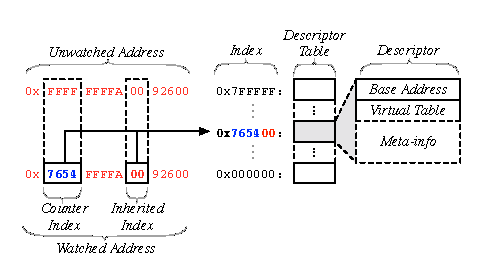
\epsfig{file=watchpoints.eps, width=3.0in, height=1.4in}
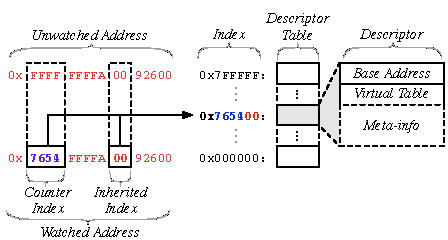
\includegraphics[width=\linewidth]{watchpoints.pdf}
\end{center}
%--------sigalternate---------- \vspace{-15pt}
\caption{\label{fig:watchpoint_descriptor_table}A watched address (bottom left) and its corresponding unwatched address (top left) are compared. The process of resolving the watchpoint descriptor is shown.}
%for the watched address is shown.}
\end{figure}

Our design is shown in \Figref{watchpoint_descriptor_table}. It uses 15 high-order bits (called the \emph{counter index}) and an additional 8 bits (bits 20-27, called the \emph{inherited index}) of a watched address to identify the index into a global \emph{watchpoint descriptor table} which stores the pointer to the watchpoint's descriptor. %This extends the number of possible watchpoints to 8M. 
The key advantage of our watchpoint scheme is the ability to directly map watched addresses to unwatched addresses using a simple bitmask. One drawback of the scheme is that an offset of a watched address can cause the low-order bits to overflow into the inherited index. We overcome this issue by assigning multiple descriptors for the watched objects holding the same meta-information and by putting them in adjacent indices. 

%is to manage multiple descriptors for a watched object.

%The watched addresses are non-canonical addresses that trigger a hardware exception when dereferenced. 
We take advantage of the x86-64 architecture for implementing watched addresses. In kernel space on x86-64, canonical addresses have their 16 high-order bits set to 1. Watched addresses do not take this form; they are non-canonical addresses that trigger a hardware exception when dereferenced. 
The watchpoint framework uses two approaches to perform memory operations on watched objects. First, when watchpoints are expected to be triggered frequently, it dynamically adds instrumentation at every memory load and store to avoid hardware exceptions. Watched addresses are detected before they are dereferenced and resolved to their unwatched counterparts (by masking the 16 high-order bits to 1). Second, when watchpoints are unlikely to be triggered, the alternative approach is to dereference a watched address and implement behavioral watchpoints in the trap handler. This enables on-demand binary translation and allows adding instrumentation only when a watchpoint gets triggered.%, which lowers the overhead of binary translation. % when watchpoints are fewer in number and unlikely to be triggered. 

Our design separates the allocation and management of descriptors from the watchpoint framework. It is the responsibility of each client to manage its descriptors. When a watchpoint gets added to an object, the client determines the \emph{vtable}, \emph{type} and \emph{meta-information} that needs to be stored in the descriptor, as shown in \Figref{watchpoint_descriptor_table}. The vtable determines the function that is invoked when watched memory is accessed. Each vtable provides eight functions: four read and four write functions. Each function is specific to a memory operand size (1, 2, 4, or 8 bytes). A watchpoint descriptor is initialized with either a generic or a type-specific vtable, which is specific to the \emph{type} of the watched address. The meta-information allows the descriptors to be arbitrarily customized or extended based on the needs of the client.


%Behavioral watchpoints earn their name from vtable because they allow watchpoints to behave differently when watched memory is accessed.

%To prevent hardware exceptions, instrumentation is dynamically added to memory loads and stores. Watched addresses are detected before they are dereferenced and resolved to their unwatched counterparts (by masking the 16 high-order bits to 1). An alternative approach is to dereference a watched address and implement behavioral watchpoints in the trap handler. This enables on-demand binary translation to selectively instrument the 


%the binary translation and instrumentation on demand, thus selectively instrumenting the code based on the usage of watchpoints. This is important when you are handling with less watchpoints and don't want to take overhead of instrumenting entire code.




%of a watched address for identifying a watchpoint's descriptor.  This extends the number of possible watchpoints to 8M.  %and is left unchanged when converting an unwatched address into a watched address.



%A watchpoint's descriptor is indirectly located by interpreting these high-order bits as an index into a global \emph{watchpoint descriptor table} which stores the pointer to watchpoint's descriptor(\Figref{watchpoint_descriptor_table}). 
%Because these bits do not change, many addresses end up indirectly referring to the same watchpoint descriptor.

%\subsection{Design Implications}
%Our approach has the following design implications.

%Any unwatched address can be converted into an watched address. The extra level of indirection added by watching an address allows us to efficiently locate context-specific information about the memory being watched.

%A watchpoint is added to a program by changing the high-order order bits of an address used by the program. 
%Watchpoints work on ranges instead of individual units of memory because a watchpoint is added to a program by changing 

%\paragraph{A watched address must be distinguishable from an unwatched address.} 

%Behavioral watchpoint framework provides API \emph{add\_watchpoints()} which is used to add watchpoints to an arbitrary object. It takes the object address and size to creates the descriptor for the object. The descriptor can be based on the type or size of the object. The descriptor can be changed dynamically if required. The descriptor is then stored into descriptor table at the next free index generated by counter and partial index. If some object doesn't need descriptor they are only assigned the watched address with corresponding index in the descriptor table assigned NULL. 

%Behavioral watchpoint provides support where two copies of an address (e.g., two pointers to the same object) can be separately watched, so long as they manage different descriptors, the high-order bits index different entries in the watchpoint descriptor table. 
%This is useful for distinguishing between logically different objects that occupy the same memory. For example, this feature enables efficient detection of use-after-free bugs without preventing deallocated memory from being immediately reallocated for another use. This efficiency comes from our ability to have one watchpoint for the freed memory, and another watchpoint for newly allocated memory occupying the same space.


%\paragraph{Multiple watchpoints can watch the same range of memory.} Two copies of an address (e.g., two pointers to the same object) can be separately watched, so long as they manage different descriptors. %the high-order bits index different entries in the watchpoint descriptor table. 
%This is useful for distinguishing between logicallywatchpoint framework  different objects that occupy the same memory. For example, this feature enables efficient detection of use-after-free bugs without preventing deallocated memory from being immediately reallocated for another use. This efficiency comes from our ability to have one watchpoint for the freed memory, and another watchpoint for newly allocated memory occupying the same space.

%\paragraph{Millions of watchpoints are supported.} Our design as described uses 15 high-order bits (called the \emph{counter index}) and additional 8 bits (bits 20-27, called the \emph{inherited index}) of a watched address for identifying a watchpoint's descriptor.  This extends the number of possible watchpoints to 8M.  %and is left unchanged when converting an unwatched address into a watched address.
%The key advantage of our watchpoint scheme is the ability to directly map watched addresses to unwatched addresses using a simple bitmask. The main drawback of the scheme is that an offset of a watched address can cause the low-order bits to overflow into the inherited index. One solution to overcome this problem is to manage multiple descriptors for a watched object. 

Our design allows the same range of memory to be watched differently. For example, two pointers to the same object can be watched separately, so long as they manage different descriptors. This feature is useful for distinguishing logically different objects that occupy the same memory. For example, this feature enables efficient detection of use-after-free bugs without preventing deallocated memory from being immediately reallocated for use. Having one watchpoint for the freed memory, and another watchpoint for newly allocated memory occupying the same space, is critical for this application. %Watchpoint gets added with a call to \texttt{ADD\_WATCHPOINT} which takes the reference of object and corresponding meta-information as parameter. \texttt{REMOVE\_WATCHPOINT} is used to remove watchpoint from a watched object. 

%For example, this feature enables efficient detection of use-after-free bugs without preventing deallocated memory from being immediately reallocated for another use. This efficiency comes from our ability to have one watchpoint for the freed memory, and another watchpoint for newly allocated memory occupying the same space.

Behavioral watchpoints can be used virally. If an address $A$ is watched, then every address derived from $A$ (e.g., through copying or offsetting) is also watched. This is useful for memory and taint analysis tools. For instance, a watchpoint that is added early in the lifetime of an address (e.g., immediately before the address of newly allocated memory is returned from an allocator) can persist and propagate until no more derived addresses exist.

%We are exploring several solutions to this problem.

% This counter index extends the number of possible watchpoints to 8M and is left unchanged when converting an unwatched address into a watched address. The key advantage of our watchpoint scheme is the ability to directly map watched addresses to unwatched addresses using a simple bitmask. The main drawback of the scheme is that an offset of a watched address can cause the low-order bits to overflow into the counter index. We are exploring several solutions to this problem.

% and 8 bits (bits 20-27, called the \emph{inherited index}) for identifying a watchpoint's descriptor

%of a watched address for identifying a watchpoint's descriptor. 15 bits only allows 32K watchpoints. To increase the number of watchpoints, we use an additional 8 bits (bits 20-27, called the \emph{inherited index}) in the address to index into the watchpoint descriptor table (\Figref{watchpoint_descriptor_table}). This counter index extends the number of possible watchpoints to 8M and is left unchanged when converting an unwatched address into a watched address. The key advantage of our watchpoint scheme is the ability to directly map watched addresses to unwatched addresses using a simple bitmask. The main drawback of the scheme is that an offset of a watched address can cause the low-order bits to overflow into the counter index. We are exploring several solutions to this problem.

%\paragraph{Millions of watchpoints are supported.} Our design as described uses 15 of the 16 high-order bits (called the \emph{counter index}) of a watched address for identifying a watchpoint's descriptor. 15 bits only allows 32K watchpoints. To increase the number of watchpoints, we use an additional 8 bits (bits 20-27, called the \emph{inherited index}) in the address to index into the watchpoint descriptor table (\Figref{watchpoint_descriptor_table}). This counter index extends the number of possible watchpoints to 8M and is left unchanged when converting an unwatched address into a watched address. The key advantage of our watchpoint scheme is the ability to directly map watched addresses to unwatched addresses using a simple bitmask. The main drawback of the scheme is that an offset of a watched address can cause the low-order bits to overflow into the counter index. We are exploring several solutions to this problem.

%This approach has some drawbacks when an offset of a watched address causes the low-order bits to overflow into the counter index; however, we have several solutions to this problem. 

%\paragraph{Watchpoint descriptors are context-specific.} Our design separates the allocation and management of descriptors from the watchpoint framework. It is the responsibility of each client to manage its descriptors. %, which % and declare the corresponding descriptor type for the framework. provides complete flexibility in handling it. 
%When a watchpoint gets added to an object, the client determines the \emph{type}, \emph{meta-information} and \emph{vtable} which needs to be stored in the descriptor. These descriptors can be arbitrarily customized or extended based on the needs of the client. %One powerful application of this extension is discussed in section~\ref{sec:access_policies}.




%This aspect of watchpoints is possible because our design separates the allocation/management of descriptors and the addresses that they watch. When a watchpoint is added to an address, the \emph{type} or \emph{size} of the address determines what meta-information is included in the descriptor, as well as what function to invoke when memory watched by the watchpoint is accessed. These descriptors can be arbitrary customized or extended based on the needs of program analysis tools. Two powerful applications of this extension are discussed in \Secref{type_overflow} and \Secref{access_policies}.


%Arbitrary extension of descriptors supports our goal of overcoming the incongruency between the needs of debugging an analysis tools (contextual information about watched memory), and how existing software implements watchpoints (watched memory is opaque).

%\subsection{Extensions}
%Our design includes the following extensions to watchpoints, which expand on the behavioral aspect of our watchpoint implementation.
%principally enable the \emph{behavioral} aspect of our software-based watchpoint .
%Our goal of using watchpoints to watch the memory of objects required the following 

%\paragraph{Watchpoints are type-specific.} When a watchpoint is added to an address, the \emph{type} of the address determines what meta-information is included in the descriptor, as well as what functions to invoke when memory watched by the watchpoint is accessed. Two powerful applications of this extension are discussed in \Secref{type_overflow} and \Secref{access_policies}.

%\paragraph{Triggered watchpoint functions are polymorphic.} The function invoked when watched memory is accessed is decided using a descriptor-specific \emph{vtable}. Each vtable provides eight functions: four read and four write functions. Each function is specific to a memory operand size (1, 2, 4, or 8 bytes). A watchpoint descriptor is initialized with either a generic or a type-specific vtable, which is specific to the \emph{type} of the watched address. %Behavioral watchpoints earn their name from vtable because they allow watchpoints to behave differently when watched memory is accessed.

%When invoked, a vtable function operates on the watched address and its descriptor. Behavioral watchpoints earn their name from their ability to behave differently based on the meta-information stored in the descriptor and the (type-specific) vtable function invoked.

%\paragraph{Watchpoints remember their originating address.} The address to which a watchpoint is first added is called its \emph{base address}, and is stored in the watchpoint descriptor. We designed watchpoints to remember their base address because it helps to ``anchor" contextual information. When a watchpoint is added, \emph{something} is known about the watched address. Later in a program's execution, an offset of the watched address might be dereferenced. Little can be said about the dereferenced address in relation to the watchpoint's originating address without knowing the originating address.

%Without the former context of why or where the watchpoint was originally added, there is little that can be said about the relation between the triggered address and 
%the watched memory except that it might be arbitrarily far away from the address to which the watchpoint was originally added.
%That is, something is known about an address when the decision to add a watchpoint to that address is made. 
%If the original address is not remembered, then it is difficult to relate a triggered watchpoint
%We designed watchpoints this way so that at any point during the lifetime of a watchpoint, 
%Watchpoints were designed this way so that contextual information is always ``anchored" to something that was once known. 

%This is consistent with our goal of using watchpoints to watch the memory of an object because we expect the base address to be the address in memory of a watched object.

%Watchpoint desc

%Because watchpoints are added to addresses, and 

%This means that 


%We can change an address into a \emph{watched address} by ensuring that a watched address is non-canonical: it cannot legally be used (on x86) without triggering a hardware exception.


%changing part of an address, not by 
%The watched range is \emph{anchored} on the address on which the watchpoint is initially added (called the base address). 

%Behavioral watchpoints are implemented by changing an address to-be-watched into a non-canonical address\footnote{In kernel space on x86, a canonical virtual address has its 16 high-order bits set to 1. Current x86 processors require that the 8 high-order bits of an address match the $9^{th}$ highest order bit.}. The translation from unwatched to watched alters the unused high-order bits of an address. 

%There are several implications of this design decision:
%\begin{enumerate}
%	\item 
%\end{enumerate}



%Behavioral watchpoints were designed with the following goals in mind:
%\begin{enumerate}
%	\item 
%\end{enumerate}

%\subsection{Design Challenges}
%The design of behavioral watchpoint put following restrictions in the way it can be used:
%\begin{enumerate*}
%\item[i)] A watchpoint must be added at the object source. Adding watchpoints at arbitrary location must be avoided since there is a possibility of another unwatched copy of the same object existing in the program data. This will introduce inconsistency and object will be partially watched.
%\item[ii)] Behavioral watchpoints can't be used in applications playing with high-order bits. Such operation will introduce inconsistency in descriptor information attached with watched addresses. Applications doing similar things like depending on sign-extension of the 64-bit addresses or handling of 32-bit addresses is also not supported. Identifying and ignoring such cases is a problem and we are exploring solutions to this.
%\item[iii)] Behavioral watchpoints are implemented for Linux kernel and one should be careful when using page-table lookup for watched addresses. Operations such as \texttt{\_\_pfn\_to\_page} and \texttt{\_\_page\_to\_pfn} can lead to wrong \texttt{page} structure or loss of descriptor information.
%One should also be careful when using kernel functions for page-table lookup on watched addresses.
%We found some cases where fast method of mapping virtual addresses to physical addresses for page table lookup was depending on sign extension of 64-bit addresses which is not the case when it is changed to watched addresses. 

 %can't be used in applications playing with high-order bits. Such operation will introduce inconsistency in descriptor information attached with watched addresses. Applications doing similar things like depending on sign-extension of the 64-bit addresses or handling of 32-bit addresses is also not supported. Identifying and ignoring such cases is a problem and we are exploring solutions to this.
%\end{enumerate*} 

%put some restrictions on the range of applications which it can handle. Behavioral watchpoint tags the higher-order bits with the descriptor information and it can't handle the application which is also doing similar things. Such operation will corrupt the embedded descriptor information and once lost we don't have a way to recover it. Identifying applications doing such operation is challenging. Applications which are only handling with 32-bit address is also not supported. We designed behavioral watchpoints for the Linux kernel but all the functionalities in the kernel is not very suitable for the approach. We found some cases where fast method of mapping virtual addresses to physical addresses for page table lookup was depending on sign extension of 64-bit addresses which is not the case when it is changed to watched addresses. 

%has the following design implications. 

%are designed for Linux kernel and generated by providing an extra-level of indirection and storing the descriptor information in higher order bits of the address. This puts restrictions on the range of applications which behavioral watchpoints can handle. The applications storing tagging information with the high-order bits of the address works against the design of behavioral watchpoints. Identifying such operations in an application is an open problem for us. Our solution of embedding descriptor information in object address is not very friendly with some of the kernel functions.   


%However identifying such operations in an application is an  


%However all the applications  


%The operation is not very friendly with some of the kernel functions. Linux kernel uses fast method of mapping virtual addresses to physical address. The mapping functions performs bit-operations in the  


%and virtual address into struct pages for lookup in the page table. 


 %to the physical address. These operations 


%There is a requirement for Linux to have a fast method of mapping virtual addresses to physical addresses and for mapping struct pages to their physical address. Linux achieves this by knowing where, in both virtual and physical memory, the global mem_map array is because the global array has pointers to all struct pages representing physical memory in the system. All architectures achieve this with very similar mechanisms, but, for illustration purposes, we will only examine the x86 carefully. This section will first discuss how physical addresses are mapped to kernel virtual addresses and then what this means to the mem_map array.   

%\subsection{Architecture}

%The implementation of behavioral watchpoints distinguishes between watched addresses and their descriptors.

%A \emph{watched address} is a pointer with an index into the \emph{watchpoint descriptor table} embedded in its bits (\Figref{watchpoint_descriptor_table}). The $23$-bit index into the descriptor table is formed by concatenating bits $[20,27]$ (called the \emph{counter index}) with bits $[48,62]$ (called the \emph{partial index}). A watched address and its unwatched counterpart share the same counter index; however, the partial index of a watched address varies\footnote{This feature of watchpoints allows for a one-to-one mapping between a watched and unwatched address, and a one-to-many mapping between a watchpoint and all addresses watched by that watchpoint. The one-to-one mapping is formed by masking the high-order bits containing the partial index.}. Partial indexes are recorded in the \emph{partial index counter table}. When a watchpoint is allocated, the current value stored in the counter table for that specific counter index is incremented and returned as the watchpoint's partial index. This allocation strategy allows for at most $2^{15}$ watchpoints per counter index or megabyte of memory\footnote{x86 has byte-addressable memory. The counter index begins at bit $20$, giving each watchpoint $1$ MB = $2^{20}$ B degrees of freedom. However, if an over/underflow across the 1 MB-aligned boundary occurs then the counter index will be corrupted. We can correct one bit of corruption by requiring that the counter index and the partial index have the same sign. An alternative solution is uses a different indexing scheme. We have successfully experimented with a different indexing scheme that solves the aforementioned overflow errors, but sacrifices the one-to-one relationship between a watched and unwatched address.}.

%A \emph{watchpoint descriptor} is a data structure containing a base address, a pointer to a virtual table (vtable) of memory operations, and programmer-defined meta-information. 


\section{Implementation}
%Granary is a DBT framework that is under development. Its primary novelty is its ability to efficiently instrument arbitrary, binary Linux kernel modules without imposing overhead on the kernel. 
We implemented behavioral watchpoints using Granary, a dynamic binary translation (DBT) framework \cite{GranaryAtOSDI}. Granary instruments arbitrary, binary Linux kernel modules efficiently and without imposing overhead when the core kernel is running. Our aim is to use Granary to analyze and debug kernel modules, which are a frequent source of vulnerabilities in operating systems \cite{BGI,LXFI}.

Granary is unique among DBT systems because it analyzes and uses program type information. For example, Granary can substitute the execution of a function with a \emph{wrapped} version of itself. A wrapped function has the same type specification as its unwrapped counterpart and can freely modify its arguments and return value. Granary can wrap some module functions in this way, even if the module source code is unavailable.

While Granary provides a framework for instrumenting kernel modules, we found it was hard to write powerful instrumentation code using low-level DBT abstractions, which motivated the design of behavioral watchpoints. Next, we describe examples of watchpoint-based debugging applications developed for kernel modules.

%We are developing Granary as a framework for building kernel module analysis and debugging tools. Analyzing kernel modules is important because they extend the functionality and bug count of operating systems [TODO CITATION]. However, analyzing module behavior is challenging. Static analysis of module source code is difficult because of the tight interaction between modules and the kernel. Some modules, however, are only distributed in a binary format, which can make static analysis intractable (on x86).



%A watchpoint is added to a previously unwatched pointer by adding an entry to the watchpoint descriptor table and embedding part of the index of the entry in the high-order bits of the pointer. The original value of the pointer is saved as the base address of the descriptor. A watchpoint is removed from a pointer by masking the high-order bits containing the partial descriptor index. This approach permits a one-to-one mapping between a watched address and its unwatched counterpart, while allowing a single descriptor to watch many addresses. Specifically, a single watchpoint can watch up to $2^{20}$ distinct addresses, and each megabyte of memory can be watched by up to $2^{16}$ distinct watchpoints.

%Watched addresses, however, do not reference valid memory. Dereferencing a watched address triggers a hardware exception. To avoid this, we use Granary to dynamically translate memory loads and stores to first check for and then resolve watched addresses to their unwatched counterparts. If a watched address is detected then a watchpoint-specific vtable function is invoked. Both the address of the watchpoint descriptor and the watched address are passed as arguments to the invoked function. Finally, the original memory instruction is emulated by one that uses the unwatched address. The choice of which vtable function to invoke depends on the size of the memory operand (1, 2, 4, or 8 bytes) and whether the operation reads or writes its operand from/to memory.


\section{Applications}\label{sec:applications}
The following sub-sections describe four applications of behavioral watchpoints and their implementations. In these sub-sections, we use the term \emph{object} to refer to a range of memory locations that are allocated together.% as a unit.

%to describe a value or aggregate of values stored in memory and referenced by a memory address.

\subsection{Buffer Overflows}\label{sec:buffer_overflows}
A buffer overflow occurs when a program---in an attempt to write to some object's memory---actually writes to adjacent memory cells. One method of detecting buffer overflows relies on the compiler to allocate ``poisoned" regions of memory around each object \cite{AddressSanitizer}. Small overflows (e.g., off-by-one errors) are detected by this approach because they access poisoned memory. Big overflows that ``skip" over poisoned memory and access nearby objects in memory are not detected.

Our insight is that unrelated objects will have different base addresses (i.e., the address of one object will not be derived from the base %address of another), and therefore a watched object can be adjacent to a different un/watched object without conflict.
address of another), and thus each object can be distinguished and uniquely identified with a separate watchpoint address%, even when objects are adjacent to each other.
%to an unwatched one, or one with a distinct watchpoint, without conflict.
%\emph{addresses} stored in hardware registers, like high-level programming language variable names, are typically not used to simultaneously access two unrelated objects.
%Accessing poisoned memory is an error because it does not exist as a named program entity. However, 
%Our approach is similar in that memory adjacent to a watched object is considered poisoned; however, we do not rely on compiler support, nor do we allocate or mark poisoned memory as such.

\begin{figure}
\begin{lstlisting}[language=C,basicstyle=\footnotesize\ttfamily]
FUNC_WRAPPER(__kmalloc, (size, flags), {
  void *addr = __kmalloc(size, flags);
  ADD_WATCHPOINT(addr, size);
  return addr;
})
\end{lstlisting}
%--------sigalternate----------  \vspace{-10pt}
\caption{\label{fig:kmalloc_wrapper}Definition of the \texttt{\_\_kmalloc} function wrapper in Granary. The above code expands into a function for wrapping the \texttt{\_\_kmalloc} allocator. Calls to \texttt{\_\_kmalloc} are transparently substituted with calls to the generated wrapper. The wrapper invokes the original \texttt{\_\_kmalloc} function and returns a watched version of the allocated address.}
\end{figure}

We employ two overflow detection policies: heap-based, and stack-based. % All three policies depend on the same extension to the meta-information of watchpoint descriptors: a \emph{limit address}. Together, the base address (stored in the descriptor) and the limit address delineate an object's boundaries in memory \cite{BccFatPointers}.


\paragraph{Heap-based overflow detection}\label{sec:heap_overflow} The heap-based detection policy detects buffer overflow errors on all heap-allocated objects. We use Granary to wrap the kernel's memory allocators (e.g., \texttt{kmalloc}) and add watchpoints to the addresses returned by those allocators, as shown in \Figref{kmalloc_wrapper}. The lifetime of an added watchpoint is tied to the lifetime of the memory it watches. Each watchpoint's descriptor records bounds information about the allocated memory in the form of the object's base and limit address \cite{BccFatPointers}. A buffer overflow is detected when a dereference of a watched address occurs outside of the bounds recorded by the watchpoint's descriptor. %(\Figref{detect_overflow}). 
The memory operand-size-specific vtable functions help catch corner cases where memory reads or writes access both an object and its adjacent memory cells.%, as shown in case $(3)$ of \Figref{detect_overflow}.

%intersect an object's memory and the adjacent memory cells.
%The vtable functions used by these watchpoints detects buffer overflows when a dereference of a watched address 
%memory dereferenced in a read or write falls outside of the bounds
%We use Granary to substitute invocations of the kernel's memory allocators (e.g. \texttt{kmalloc}) with wrapped versions of the allocators (\Figref{kmalloc_wrapper}). A wrapped allocator invokes the original allocator but returns a watched version of the allocated address. The lifetime of the watchpoint is 
%The watched address returned has its descriptor initialized with the base address as the allocated address and with the limit address as the base address plus the requested allocation size. All buffer overflow detecting watchpoints are initialized with the same vtable pointer.
%The vtable pointer used by all buffer overflow detecting watchpoints points to a table of memory operand size-specific functions. The operand size is necessary to detect dereferences of memory that overlap both the object and its adjacent memory, as illustrated in case \emph{(3)} of . The vtable function corresponding to the memory operand size is invoked when a watched address is dereferenced. Each vtable function is programmed to check the watched address against the base and limit addresses stored in watchpoint's descriptor (\Figref{detect_overflow}). If a buffer underflow or overflow is detected then the vtable function notifies the run-time system.

%\begin{figure}
%\abovedisplayskip=0pt
%\belowdisplayskip=0pt
%\begin{center}
%	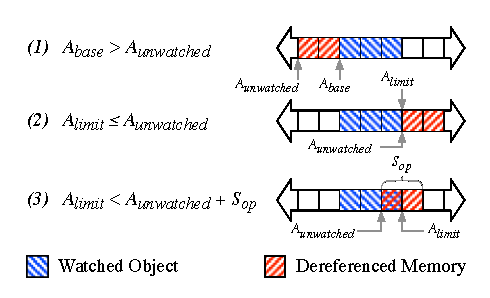
\epsfig{file=overflow.eps}
%\end{center}
%\iffalse
%	\abovedisplayskip=0pt
%	\belowdisplayskip=0pt
%	\begin{align*}
%		A_{base}  & > {A_{unwatched}} \tag{Underflow} \\
%		A_{limit} & \leq {A_{unwatched}} \tag{Overflow} \\
%		A_{limit} & < {A_{unwatched}} + S_{op} \tag{Overlap}
%	\end{align*}
%\fi
%\caption{\label{fig:detect_overflow}Three common buffer overflow cases are illustrated above: 1) underflow 2) overflow, and 3) overlap. Beside each illustration is the policy that detects the specific bug. When a watched address ($A_{watched}$) is dereferenced, a vtable function that is specific to the memory operand size ($S_{op}$) is invoked. This function detects a buffer overflow if the intended referenced memory address ($A_{unwatched}$) does not fall within the boundaries delineated by the base and the limit addresses ($A_{base}$ and $A_{limit}$, respectively).}
%\end{figure}

%\paragraph{Type-based overflow detection\label{sec:type_overflow}}
%Type-based overflow detection is applied when the type of an object is known. It is distinguished from heap-based overflow detection in that it can apply both to heap and non-heap memory, and it can be used to inform the run-time system about more accurate bounds information. In all other respects, the type-based overflow detection policy detects bugs in the same way as the heap-based policy.% (as might be encoded within the fields of a vector-like data structure).

% If the type of an object is known then it can reveal semantic relationships which can enable further type- or heap-based overflow detection. For example, the fields within a structure might encode memory bounds information (as would be the case for a vector-like data structure)

%The type-based detection policy is applied when the type of a pointer is known (i.e., not \texttt{void*}). The simplest use case of type information is to infer the limit address of a typed pointer. A more complex use case arises when the fields within a structure encode memory bounds information. In both cases, the vtable functions for typed and untyped memory operate in the same way.

%The type of an addressable object becomes known to Granary in the context of a wrapped function. The run-time system performs a type-specific initialization of a watchpoint's descriptor when a watchpoint is added to a pointer/address with a known type. Type-specific descriptor initialization is a powerful feature because it allows for new watchpoints to be lazily added (thus propagating our detecting capabilities) to newly discovered objects referenced \emph{within} an object of a known type. We automatically propagate type-based watchpoints using type specifications generated from parsing \texttt{C} header files. %Some manual post-processing is required if one is to inform the system of semantic relationships between function arguments or structure fields.

%use a type-specific vtable instead of a generic vtable when watching a typed pointer. Granary includes a database of 


%Granary recursively follows argument and return value pointers based on object type specifications. These specifications tell Granary how to follow pointers and what--if any--pointers should be converted to watchpoints. To reduce programmer effort, Granary automatically generates type specifications and wrapper functions for any set of known types and functions. Some manual post-processing is required if the analysis/debugging application needs to understand semantic relationships between function arguments or structure fields. \comment{Automating this process was an important goal of Granary because of Granary wraps all (approx. 6,000) exported kernel functions.}


%We detect overflows on stack allocated objects when memory outside of the bounds of the activation/call frame in which the object is allocated is accessed. This policy is distinguished from the heap- and type-based policies in that the watchpoint descriptor is managed separately from the watched memory, and the lifetime of the descriptor extends beyond the lifetime of the watched memory.

\paragraph{Stack-based overflow detection} To detect stack overflows, we view the memory occupied by the activation frame of an invoked function as a dynamically-sized buffer. %Like our other buffer overflow policies, we use a watchpoint to detect accesses to memory outside of this buffer. %Unlike our other policies, %we only \emph{associate} a descriptor with this buffer, and rely on a different mechanism to \emph{add} the watchpoint to stack addresses.
%, and manage what addresses are watched with this descriptor using a separate mechanism.
%We separate adding watchpoints from allocating descriptors for stack overflow detection. In particular, 
We associate a descriptor with the buffer represented by the activation frame of a called function. This descriptor tracks the bounds of the frame over the lifetime of the function call.

We update the bounds of the frame (in the descriptor) when the frame grows or shrinks. When a function returns, the descriptor's bounds shrink to zero, but the descriptor remains allocated. We detect the two most common sources of stack overflows. First, if we see an instruction that copies the stack or frame pointers, then we assume that the copied address can escape the function. A stack address escaping a function is a potential stack-overflow risk. Adding the frame's watchpoint to this address \emph{taints} the copied address. Future copies or displacements of the watched address implicitly propagate its taintedness because offsets of a watched address reference the same descriptor. A dereference of an escaped pointer---even one happening after the function has returned---is detected as an overflow because the watchpoint descriptor remains live. Second, if we see an indexed dereference of the stack or frame pointers that uses a dynamically bound index, then we assume that the effective memory address accessed is a potential stack-overflow risk. We instrument the dereferencing instruction to add the frame's watchpoint to the effective address before the address is dereferenced.

%and addresses that we want to have watched by 
%Under this lens, we associate a watchpoint descriptor with each function call that tracks the bounds of each activation frame. 
%allocating one watchpoint descriptor for each function call. This descriptor exists to track the bounds of the activation frame over the lifetime of the function call. The run-time system dynamically adds instructions to the instrumented program that change the recorded bounds when the size of the activation frame grows or shrinks. When a function returns, the descriptor's bounds shrink to zero.

%Instrumentation is dynamically added to the program that increase/decrease the recorded size of the activation frame in the descriptor when the 
%The descriptor tracks the size of the activation frame

%Unlike the heap- and type-based overflow policies, there are numerous optimizations 
%Stack-based overflow detection is distinguished from the heap- and type-based policies in that numerous optimizations are possible, and that 
%in an access to memory outside of the object's activation frame.
%The aforementioned approaches to overflow detection 
%Stack-based overflow detection is distinguished from the heap- and type-based overflow detection policies insofar as it uses 

%Detecting stack overflows is important because they are commonly used in remote code execution and privilege-escalation attacks against operating systems \cite{SecureProgramExecFlowTracking}.

% more support from Granary's run-time system. At a high level, each activation frame is assigned a dedicated watchpoint when a function is called. The effect of an instruction that grows or shrinks an activation frame's size is reflected by a similar change to the base address\footnote{The run-time call stack on x86 grows into lower memory.\comment{ Modifying the base address instead of the limit address allows us to maintain one set of vtable functions for all three buffer overflow detection policies.}} of the frame's watchpoint descriptor. When a function returns, the descriptor of its activation frame is cleared, but remains allocated\footnote{Reclaiming/reusing allocated but unlikely-to-be-used watchpoints is challenging. One overflow-specific approach is to ensure that the next use of the watchpoint is for a buffer whose bounds do not intersect with the current use's bounds. Another approach is to use some number of context switches as a grace period in which the watchpoint cannot be reused, but after which it can be reused. We leave this as future work.} lest the address of a local variable escape the function\footnote{If the address of a stack-allocated object escapes its function activation frame, then that pointer is said to be \emph{dangling}. Dereferences of dangling pointers can cause stack overflow errors. In the kernel, data stored in unallocated stack memory (e.g., through a dangling pointer) is at risk of being clobbered by interrupt stack frames and by function activation frames.}.  

%We assume that a memory instruction operating on a constant displacement of the stack or frame pointer registers is well-behaved. However, if the stack or frame pointer registers participate in a memory instruction and the displacement from the register is dynamically-bound then that instruction is suspect. An instruction that copies the address in the stack or frame pointer registers is also suspect because the copied address might escape the current function or participate in a local stack overflow. All suspect instructions are translated to transparently add the frame's dedicated watchpoint to the dereferenced or copied address.

%This scheme segments the runtime stack into contiguous but non-overlapping regions of watched memory. A straightforward extension excludes saved return addresses and link pointers from the known bounds of activation frames, thus detecting return-oriented buffer overflow attacks.

\subsection{Selective Memory Shadowing}\label{sec:uninitialised_memory}

In this section, we show how to use behavioral watchpoints to shadow memory. Previous work has focused on full memory shadowing \cite{Memcheck}, while watchpoints enable \emph{selective} shadowing of watched objects. We describe how the initialization state of each byte of watched memory is tracked using shadow memory, and how to detect bugs related to the usage of heap-allocated memory.

We use Granary to wrap kernel memory allocators and deallocators (e.g., \texttt{kmalloc}, \texttt{kfree}). Wrapped allocators add watchpoints to allocated memory, and wrapped deallocators remove watchpoints before invoking the kernel's deallocators. Selective shadow memory is maintained as a watchpoint descriptor-specific, variable-sized bitset. Each byte of allocated memory corresponds to one bit of shadow memory. The bits in shadow memory are initialized to zero. Individual bits are flipped to one by injected instrumentation code  when a write occurs to the memory shadowed by those bits.

%write-specific instru functions when there is a write to the bytes of memory shadowed by those bits. 

%When a wrapped allocator is invoked, a watchpoint is added to the addresses returned by those allocators
 

% in shadow memory are initialized to zero.
%Watchpoints are added to all heap-allocated objects 
%the meta-information within each watchpoint descriptor.
%By tracking the initialization state, we detect


%We apply the above shadow memory scheme to detect uses of uninitialized memory for heap-allocated objects. As in \Secref{heap_overflow}, we interpose on the kernel's memory allocators and add watchpoints to the addresses returned by those allocators. When memory is allocated, the watchpoint descriptor is initialized with the number of allocated bytes (available as an argument to the allocator) and with its own shadow memory. 

%detect uses of uninitialized memory.  Detecting such uses is important because a program using uninitialized memory can exhibit unintended, non-deterministic behavior.

%We define uninitialized memory as either allocated memory to which no value has been written, or de-allocated memory. We selectively track the initialization state of each byte of watched memory using \emph{shadow memory} \cite{Memcheck}. Our implementation represents shadow memory as a bitset, where the state of each bit tracks the initialization state of a byte of watched memory. Watchpoint descriptors are augmented to include the size (in bytes) of a watched object and a pointer to the memory shadowing the object\footnote{As an optimization, shadow memory for small objects can be embedded in the watchpoint descriptor.}.



\paragraph{Read-before-write bugs} Memory read instrumentation detects read-before-write bugs by checking if the shadow bit corresponding to one of the read bytes is zero. However, this method of detection can report false positives: it is common for larger-than-needed reads to be performed and for compiler-added structure padding to be read (but never written). A relaxed read-before-write memory checking policy requires that at least one shadow bit is set for every read operation.

% We detect freeing of non-heap memory when the argument to a kernel memory deallocator is not a watched address. 

\paragraph{Memory freeing bugs} 
An invalid free bug occurs when an object passed to a deallocator was not 
previously obtained from an allocator. For example, this may happen if an offset of an allocated object is freed instead of the original object. We detect invalid frees when the freed address doesn't match the base address of the watched object.
We detect use-after-free bugs by marking the descriptor of a watched address being deallocated as dead. The lifetime of a dead descriptor extends beyond that of the object so that a later use of any watched address with that descriptor will report a use-after-free bug. We detect double-free bugs when the descriptor of a watched address being deallocated is already marked as dead.

%We use Granary to wrap the kernel's deallocation functions (e.g., \texttt{kfree}). Because all allocators are wrapped and add watchpoints, freeing of non-heap memory is easily detected when  

%We detect freeing of non-heap memory 

%If the argument to a wrapped deallocator function is a watched address then the shadow memory for the . 

%Finally, the original deallocator is invoked with the unwatched address as an argument. Reads and writes to a watched address of a deallocated object fail to pass bounds checks because the object size is zero.

%Two positive side-effects of our approach is that it detects double-free bugs and freeing of non-heap memory bugs. A double-free is detected when a watched address for an already deallocated object is passed as an argument to a deallocator. An attempt to free non-heap memory is detected when an unwatched address is passed as an argument to a deallocator.

\subsection{Memory Leak Detection}\label{sec:memory_leaks}
We built a memory leak detector for module-owned objects. A module is responsible for deallocating such objects. Not all module-owned objects are allocated by modules. For example, \texttt{sk\_buff} objects used by network modules are allocated by kernel interrupt handlers, but must be deallocated by the network modules. Our approach ensures that all module-owned objects are watched when allocated.

The leak detector scans kernel memory using the conventional mark/sweep algorithm \cite{Boehm:1991:MPG:113445.113459} to detect if/when module-owned objects become unreachable starting from a set of ``root'' objects. This is challenging because modules regularly lose internal references to the objects that they own. For example, a network module can allocate objects and pass them t othe kernel with the \texttt{net\_device} structure, without retaining references to those objects. The network module can later indirectly access these objects using the kernel's \texttt{netdev\_priv} interface. Tracking the liveness of these objects requires a view on kernel execution not normally provided by module-only instrumentation. Behavioral watchpoints solve this problem by giving the leak detector visibility into kernel accesses to watched objects, which trigger hardware traps that attach instrumentation to the kernel code. This instrumentation marks kernel-accessed watched objects as live.

The leak detector benefits from using watchpoints in three ways: \begin{inparaenum}[i)]
	\item watched addresses are easily disambiguated from normal memory addresses and integers that look like watched addresses;
%        \item the scope of scanning can be limited using the meta-information provided by descriptors
	\item descriptors provide meta-information that allows our system to limit the scope of scanning; and
	\item scanning can stop if all watched objects are reached.
\end{inparaenum}

%Two key benefits of our watchpoints solution is that watched addresses are easily disambiguated from normal memory addresses, and that we can stop scanning memory if all watched objects are live and reachable.

%Detecting leaks of such objects with a limited view of module is challenging. Behavioral watchpoints provide a way to ensure the visibility of such objects by triggering a hardware trap on its access and mark them as live.
%on memory access of these objects by enabling demand-based translation and marking them as live.


% during device registration. 


%The object becomes invisible to the module and gets accessed through the kernel interface \texttt{netdev\_priv}. This makes it difficult to detect leaks based on module's limited view. Behavioral watchpoints provides a way to ensure complete visibility on memory access of these objects by enabling demand-based translation and marking them as live.

%All module owned objects are not directly allocated by the module and kernel can allocate it on behalf of the module. 
%All module-owned objects are not directly allocated by the module. For example, a network driver module may make a call to an skb allocator (to allocate a \texttt{sk\_buff} structure) in an interrupt context. Once the buffer is send over the network, it is the responsibility of the network module to deallocate the buffer. In Granary, we use wrappers to add watchpoints at relevant allocators such as \texttt{\_\_alloc\_skb}. The leak detector keeps track of these watched objects and reports possible leaks. 

%Module holds partial view of the kernel and to detect leaked object there is a need to perform reachability analysis on both kernel and module objects. Behavioral watchpoints helps in identifying the objects owned by the module, thus limiting the type of objects which needs to be tracked. Watched object holds descriptor information in high-order bits, making it easy to track the memory state information. This is helpful in identifying live objects and reduces the chance of false positive. The leak detector uses the conventional mark and sweep algorithm and mostly-parallel collector~\cite{Boehm:1991:MPG:113445.113459} to perform the reachability analysis.
 
%Watched addresses are also more easily disambiguated 

%Behavioral watchpoints are important for implementing the leak detector because they help in identifying the objects owned by the module, thus limiting the type of objects that need to be tracked. Each watched object holds the memory state information embedded in its descriptor, making it easy to identify objects that are live and reachable. % from one of the root-sets\footnote{The root-set for leak detector reachability-analysis includes both kernel and module data structures.}. 
%The leak detector uses the conventional mark and sweep algorithm and mostly-parallel collector~\cite{Boehm:1991:MPG:113445.113459} to perform the reachability analysis.


%are easily identifiable because they hold the descriptor table index in high-order bits and 3) Each watched object holds the memory state information with it. Thus making it easy to identify the the objects which are live and reachable from one of the root-sets. The leak detector uses the conventional mark and sweep algorithm and mostly-parallel collector~\cite{Boehm:1991:MPG:113445.113459} to perform the reachability analysis.



%there is a need to perform reachability analysis of all kernel objects, which will have significant cost.



%then gets accessed through the kernel interface and become invisible to the module and is reachable only through the \texttt{net\_device} structure. Behavioral watchpoints ensures complete visibility of these objects and enables on-demand instrumentation on its access, marking them live.



%Developing a leak detector only for kernel modules is challenging because of following three reasons:
%Our approach is based on performing reachability analysis on module owned objects. 
%Memory leak is a common problem in Linux kernel and its modules \cite{Boehm96simplegarbage-collector-safety}. A serious memory leak in kernel modules can easily make the system unstable this is because every time kernel losses a piece of memory, it can't be reclaimed until next boot. 
%Our approach of detecting memory leaks in kernel module is to perform reachability analysis on the module owned objects. 
%This is challenging because: 

%1) All module owned objects are not directly allocated by the module. For example, a network driver module may make a call to an skb allocator (to allocate a \texttt{sk\_buff} structure) in an interrupt context when the module code is not running. Once the buffer is send over the network, it is the responsibility of the network module to deallocate the buffer.

%2) Module allocates many independent objects which they share with the kernel. Module losses its visibility once such objects are passed to the kernel. For example, a network module during device registration can allocate an object and pass it with \texttt{net\_device} structure. This object then become invisible to the module and is reachable only through the \texttt{net\_device} structure. Detecting leak for such objects requires complete visibility of the kernel. 
%an object and pass it with \texttt{net\_device} structure. 
%till it gets its reference 
% passed to the kernel till it gets his reference back. 
%frequently share with the kernel. Module looses the visibility for such objects till it gets back their references. For example, filesystem module \texttt{ext3} allocates object of type \texttt{inode} and passes it to the kernel. The module holds no reference of the object once it is passed and only 
%loose its visibility for module code till the time kernel passes them back to the module. For example,   
%There is frequent transfer of module allocated objects at kernel/module interface and module may not hold the reference of objects passed to the kernel.  For example, file-system module \texttt{ext3} allocates object of type \texttt{struct inode} and passes it to the kernel. Once it is passed to the kernel module doesn't hold reference of \texttt{struct inode}. Thus having limited view of the module doesn't help in detecting leaks.  

%3) Module only holds partial view of the kernel and much of the module allocated objects are reachable only through the kernel objects. To detect the leaked object there is a need to perform reachability analysis of all kernel objects, which will have significant cost.


%and detect the leaked objects it is needed to perform the reachability analysis on 


%In Granary, we use wrappers to add watchpoints to the relevant allocators (e.g., \texttt{\_\_alloc\_skb, skb\_clone}). The leak detector keeps track of these watched objects and reports possible leak. 

%Behavioral watchpoints are important for implementing the leak detector because: 1) They help in identifying the objects owned by the module, thus limiting the type of objects which needs to be tracked, 2) The watched addresses are easily identifiable because they hold the descriptor table index in high-order bits and 3) Each watched object holds the memory state information with it. Thus making it easy to identify the the objects which are live and reachable from one of the root-sets. The leak detector uses the conventional mark and sweep algorithm and mostly-parallel collector~\cite{Boehm:1991:MPG:113445.113459} to perform the reachability analysis. % from its root-sets. 
%Based on this leak detector divides the watchpoints into three different categories: 
%\begin{enumerate*}
%   \item[i)] Watched objects which are reachable from one of its rootset. They are not considered as leak.  
%   \item[ii)] Watched objects that are not reachable from any of the rootsets are considered as potentially garbage. 

   %Watched objects that are not reachable and never owned by the modules are considered as live. This include objects which are allocated in the module context but never reached to the module. Leak detector keeps tracks of such objects by for further analysis.
    %These includes objects which are allocated in module context but are not owned by the modules. Leak detector keep tracks of such objects by marking them as live. 
%   \item[iii)] Module owned objects that are not reachable from any of the rootsets are considered as potentially garbage. 

   %Determining the garbage objects with partial view of kernel and scanning of kernel objects passed to the module is challenging. However, to determine this we follow the ownership history of the objects and any watched objects which is owned by the modules previous and are not reachable from any of the root-sets is reported as leak. Root-sets are set of object references which are prior reachable and for our leak detector it includes kernel and module static data and kernel objects passed to the module.  
%\end{enumerate*}


%in performing reachability analysis, as the addresses are identifiable and it stores the state of a memory 



%allocation of \texttt{struct sk_buff} in interrupted context and it is the responsibility of the module to deallocate it.  


%call \texttt{__alloc_skb} in interrupted context to allocated sk


%which is passed to the module.    


%Leak detector identifies the module ownership of an object based on its context of allocation and access pattern. Performing reachability-analysis on these objects are challenging because not all module owned objects are directly allocated by them. Granary identifies the


%The module ownership of an object is identified by its context of allocation and access pattern. 

%Behavioral watchpoints track the ownership of an object by identifying its source of allocation and access pattern.


%However, 


%this is challenging because not all objects owned by the module are directly allocated by them.   

%Every time kernel losses a piece of memory, it is gone until the next boot and a serious memory leak in the kernel modules can easily make the system unstable. One method of detecting memory leak in kernel modules is to perform reachability analysis on all allocated objects. This is challenging because not all module owned objects are directly allocated by the module and there is frequent transfer in ownership of the objects at kernel/module interface.

%Behavioral watchpoints track the ownership of an object by identifying its source of allocation and access pattern. To detect the memory leak, Leak detector performs reachability-based analysis only on the objects owned by the module. Study of object ownership also helps in fixing the responsibility for deallocating the object and any default in this is considered as memory leak.

%We use Granary to wrap the kernel’s memory allocator functions (e.g., \texttt{\_\_kmalloc}) and add watchpoints to the objects allocated in the module context. It decides this based on the call graph of the allocator functions. Granary also tracks the kernel objects passed to the module at interface and mark them as module known objects. Leak detector use these module known objects along with kernel and module static data as rootset to perform reachability analysis. Other alternative for reachability-analysis is to scan entire kernel heap.  

%Granary also keeps track of all the objects passed to the module at interface and considers them as root-set to perform reachability analysis. However, this approach provides leak detector limited view of the kernel and based on that it divides the allocated objects into three categories:
%\begin{enumerate*}
   %\item[i)] Module owned objects that are live and reachable from one of the prior roots are not considered as leak. 
   %\item[ii)] Watched objects that are not reachable and never owned by the modules are considered as live. This include objects which are allocated in the module context but never reached to the module. Leak detector keeps tracks of such objects by for further analysis.
    %These includes objects which are allocated in module context but are not owned by the modules. Leak detector keep tracks of such objects by marking them as live. 
   %\item[iii)] Module owned objects that are not reachable from any of the rootsets are considered as potentially garbage. 

   %Determining the garbage objects with partial view of kernel and scanning of kernel objects passed to the module is challenging. However, to determine this we follow the ownership history of the objects and any watched objects which is owned by the modules previous and are not reachable from any of the root-sets is reported as leak. Root-sets are set of object references which are prior reachable and for our leak detector it includes kernel and module static data and kernel objects passed to the module.  
%\end{enumerate*}

%for the module-owned objects.    




%is to perform the reachability analysis on all kernel allocated objects. 

%Memory leak bugs are a common problem with C and C++ based applications \cite{Boehm96simplegarbage-collector-safety}. These bugs are difficult to identify or track-down without the help of a dedicated tool \cite{Memcheck, Bruening:2011:PMC:2190025.2190067}. Memory leak can be a problem especially in long running application and is worse in the kernel because every time a piece of memory is lost, it is gone until the next boot.
%Memory leaks can be a problem in applications, especially those which run for a long time
%Memory leak bugs are common in Linux kernel and its modules which are mostly developed in C. These bugs are difficult to identify or track-down without the help of a dedicated tool. 
%Memory leaks in kernel is worse because of its long running nature and every time a piece of memory is lost, it is gone until the next boot. 
%Linux kernel modules works as an extension of Operating system providing additional features, while running in the privilege mode and a serious memory leak in the kernel modules can make the operating system unstable. In this section we will describe our approach of using behavioral watchpoints in detecting memory leak bugs in kernel modules.

%\paragraph{Liveness Analysis} Our approach of leak detector is based on the liveness analysis of heap objects, which are directly or indirectly allocated by the modules. Similar to existing solution like Purify \cite{Rs_purify:fast} and Dr Memory \cite{Bruening:2011:PMC:2190025.2190067}, leak detector uses garbage collection algorithm to detect memory leaks. %Behavioral Watchpoints being able to hold context-specific information with each objects and are equally efficient for both the methods
%It uses conventional mark and sweep algorithm and recursively follows potential pointers from the data, stack segment and heaps to mark the objects live and reachable. Many implementation of mark and sweep based tracing algorithm exist and a straightforward implementation involves stopping the client(mutator) to perform the liveness analysis. This solution is not very efficient when client operates on very large heap-memory as it will increase the pause-time and touching heap memory will blow away the cache, seriously affecting the system performance. One solution to reduce the pause time is using generational collection based algorithm. However, this avoids the problem by scheduling the collector thread less frequently, thus doesn't remove the problem completely. In our leak detector we remove this problem by using mostly parallel collector. Mostly-parallel collectors takes an orthogonal approach and reduces the problem by having collector doing most of the work parallel to the client and using stop-the-world to prepare the system. 


%running collector parallel to client

%However this doesn't completely remove the 


%. The solution to reduce the pause time in tracing algorithm based leak detector is generational or parallel collection. Generational collection avoids stop-the-world time by running the collector thread occasionally, thus doesn't remove the problem completely. However the parallel collectors takes orthogonal approach and reduces the time of pause by running collector parallel to client. We took similar approach of mostly-parallel collector to perform the object liveness analysis.  




%A straightforward implementation of tracing based collector involves stopping the client when collector is in the process performing liveness-analysis. This solution is not very efficient when client operates on very large heap-memory as it stops the clients for longer time. The solution to reduce the pause time in tracing algorithm based leak detector is generational or parallel collection. Generational collection avoids stop-the-world time by running the collector thread occasionally, thus doesn't remove the problem completely. However the parallel collectors takes orthogonal approach and reduces the time of pause by running collector parallel to client. We took similar approach of mostly-parallel collector to perform the object liveness analysis.  


%purify uses an algorithm similar to the conventional mark and sweep. In the mark
%phase,i lyify-recursively follows potential pointers from the data and stack segments in to the heap and marks all
%blocks referenced in the standard"conservative"n d "pessimistic" 

%embed context-specific information with each objects and are equally efficient for implementing both direct and indirect method of leak detection but we decided to use the tracing algorithm which has no overhead cost for maintaining and updating the records for each objects.



%both direct and indirect method of leak detection but we decided to use the tracing algorithm which has no overhead cost for maintaining and updating the records for each objects.


%The existing solution for memory leak detection uses two methods to perform liveness analysis: the reference counting \cite{Maebe_precisedetection} and tracing methods \cite{Bruening:2011:PMC:2190025.2190067}. 


%The existing solution for memory leak detection uses two methods to perform the liveness analysis: the direct method and the indirect method. Direct method requires that a record be associated with each object in the heap on behalf of the objects which gets updated based on if a pointer is set to refer to this object or the reference of the object is lost. Reference counting is one of the common direct method for detecting leaks. The indirect method includes the tracing algorithm where the live-ness analysis is performed at later point of time independent of client. Behavioral Watchpoints embed context-specific information with each objects and are equally efficient for implementing both direct and indirect method of leak detection but we decided to use the tracing algorithm which has no overhead cost for maintaining and updating the records for each objects.

%\paragraph{Leak Scan}
%A common tracing algorithm used to implement garbage collector is mark-and-sweep operation. We used similar method to perform the liveness analysis on module allocated objects. A straightforward implementation of tracing based collector involves stopping the client when collector is in the process performing liveness-analysis. This solution is not very efficient when client operates on very large heap-memory as it stops the clients for longer time. The solution to reduce the pause time in tracing algorithm based leak detector is generational or parallel collection. Generational collection avoids stop-the-world time by running the collector thread occasionally, thus doesn't remove the problem completely. However the parallel collectors takes orthogonal approach and reduces the time of pause by running collector parallel to client. We took similar approach of mostly-parallel collector to perform the object liveness analysis.  

%\paragraph{Types of Leak}
%Implementing memory leak detector for kernel modules without having full knowledge of kernel is non-trivial. This is because not all module owned objects are directly allocated by the module and there is frequent change in the ownership of the objects at kernel/module interface. Leak detector makes use of wrapper interface of Granary to add watchpoints with all the objects allocated in module context and lazily tracks their ownership at collection. This is particularly important to reduce the false positive. However, our approach of lazily determining object ownership require us to keep track of all the objects passed to the modules but this avoids the scanning of kernel heaps for liveness-analysis. Based on limited kernel view and lazy collection of objects allocated by the modules, leak detector divides them into three categories: 
%\begin{enumerate*}
%   \item[i)] Objects that are live and reachable from one of the prior roots. These objects are not considered as leak. 
%   \item[ii)] Objects that are not reachable but are potentially live. These includes objects which are allocated in module context but are not owned by the modules. Leak detector keep tracks of such objects by marking them as live. 
 %  \item[iii)] Objects that are not reachable and are certainly garbage. Determining the garbage objects with partial view of kernel and scanning of kernel objects passed to the module is challenging. However, to determine this we follow the ownership history of the objects and any watched objects which is owned by the modules previous and are not reachable from any of the root-sets is reported as leak. Root-sets are set of object references which are prior reachable and for our leak detector it includes kernel and module static data and kernel objects passed to the module.  
%\end{enumerate*}



%A root-set is de-
%fined by the set of references of objects which are prior
%reachable. 



%These are the objects that never passed directly to the kernel and also not reachable from the rootsets. Leak detector reports them as potentially leaked objects. 


% kernel and modules frequently changes the ownership of objects at complex interface.  

%This is because kernel and modules frequently changes object ownership at complex interface and not all the 


%since the modules are tightly integrated with the kernel exchanging objects at complex interface. This makes it challenging to perform the liveness-analysis. Leak detector uses partial kernel information embedded in the Granary to create the root-sets. A root-set is defined by the set of references of objects which are prior reachable. We take a conservative approach in defining root-sets and apart from the static data of the module and kernel, we include all the dynamically allocated kernel objects which are ever passed to the modules as root-set. This avoids the scanning of entire heap but the leak detector has to maintain bookkeeping of such objects. Based on limited kernel view and scanning of root-set objects, leak detector divides the heap allocated objects into three categories: i) Objects that are reachable and not garbage. These are the objects which are reachable from the root-set and not considered as leak. ii) Objects that are not reachable and potentially garbage. This includes the objects which are directly or indirectly allocated by the modules but are passed to the kernel at some point. Leak detector consider it as a potential object for leak and reports them if large number of such objects exist. iii) Objects that are not reachable and are certainly garbage. These are the objects that never passed directly to the kernel and also not reachable from the rootsets. Leak detector reports them as potentially leaked objects. 


%Memory chunks that are certainly garbage and need to be reclaimed.
%Memory chunks that are potentially garbage.
%Memory chunks that are not garbage. 



 %liveness-analysis on the heap allocated objects divides the scanning objects into three categories: i) Memory that is reachable by the root-sets. This is considered as live and acts as the root-set to perform the reachability on other objects.


 %Many applications do not explicitly free memory whose lifetime matches the process lifetime and this is not considered an error. 

%Performing reachability analysis on the 
%For performing the reachability analysis on the heap allocated objects, the leak detector divides the scanning objects into three categories: i) Memory that is still reachable by the application. This is not considered a leak. Many applications do not explicitly free memory whose lifetime matches the process lifetime and this is not considered an error. ii) Memory that is definitely not reachable by the application
%(at least, not by an aligned pointer to the start or middle of the allocated block). This is called a leak as there is no way for the application to free this memory: it has lost all references to it. iii) Memory that is reachable only via pointers to the middle of the allocation, rather than the head. This is called a possible leak. These may or may not be legitimate pointers to that allocation.

 %The parallel collector imposes overhead on the mutator but it eliminates long pause due to stop the world. While designing the collector we took middle approach and used mostly parallel tracing collector to perform the reachability analysis. We update the root-set in stop-the-world collector and perform the reachability analysis on these rootsets by running collector parallel to the mutators.



 %concentrate on reclaiming recently allocated objects and it reduces the stop-the-world pause time by running the collector occasionally in-order to perform the reachability analysis on older objects. Thus, the problem of stop-the-world is not completely removed.


 %Generational collection concentrate on reclaiming recently allocated objects and it reduces the stop-the-world pause time by running the collector occasionally in-order to perform the reachability analysis on older objects. Thus, the problem of stop-the-world is not completely removed. Parallel collectors takes orthogonal approach and reduces the time of pause by running it parallel to the mutator(client). The parallel collector imposes overhead on the mutator but it eliminates long pause due to stop the world. While designing the collector we took middle approach and used mostly parallel tracing collector to perform the reachability analysis. We update the root-set in stop-the-world collector and perform the reachability analysis on these rootsets by running collector parallel to the mutators.




%However the tracing technique also suffers from some drawbacks and one of them is long delay in performing the object liveness analysis. One of the approach to smoothly detect the memory leak using tracing technique is to concurrently perform the liveness analysis.

%or root that object is reachable. A most common direct method of garbage detection/collection is the reference counting. In this method each object is associated with the reference count which gets incremented when a pointer is set to refer to this object and is decremented when a reference of the object gets deleted. The reference counting mechanism is advantageous in the sense that the memory management overhead in this case gets distributed throughout the program execution but it is weak in resolving cycles and collecting the cyclic data structure.  The other indirect method includes the tracing algorithm for garbage collection. The tracing algorithm based garbage collector maintains a set of roots and periodically perform the reachability analysis to check the liveness of the objects. The tracing technique has an advantage over the reference counting is that no precaution is needed while handling cycles and also the overhead for maintaining and updating the records(reference counting) is not there.   


% developed in C or C++ and can be difficult to identify without the help of a dedicated tool. The problem is particularly important in applications which run for a long time. Memory leak in kernel is worse because of its long running nature and every time a piece of memory is lost, it is gone until next boot. In this section we will describe our approach of using behavioral watchpoints in detecting memory leak bugs in kernel modules. Linux kernel module is a software component which extends the functionality of Operating system. Once loaded these modules executes in privilege mode having full control on the kernel resources and a serious memory leak in the kernel modules can make the system unstable.

%Our approach of leak detection is based on the reachability analysis of heap objects, directly or indirectly allocated by the modules, as opposed to considering unfreed memory as a leak. This is similar to tracing garbage collector’s mark-and-sweep operation. A straightforward implementation of tracing garbage collector algorithm involves stopping the client when collector is in the process performing liveness-analysis. This solution when applied with mutators operating on very large heap is not very efficient. This is one of the primary argument against using the tracing algorithm in memory leak detection. The other solution to reduce the pause time in tracing algorithm based leak detector is: i) generational collection ii) parallel collection.  Generational collection concentrate on reclaiming recently allocated objects and it reduces the stop-the-world pause time by running the collector occasionally in-order to perform the reachability analysis on older objects. Thus, the problem of stop-the-world is not completely removed. Parallel collectors takes orthogonal approach and reduces the time of pause by running it parallel to the mutator(client). The parallel collector imposes overhead on the mutator but it eliminates long pause due to stop the world. While designing the collector we took middle approach and used mostly parallel tracing collector to perform the reachability analysis. We update the root-set in stop-the-world collector and perform the reachability analysis on these rootsets by running collector parallel to the mutators.

%Performing reachability analysis on the 
%For performing the reachability analysis on the heap allocated objects, the leak detector divides the scanning objects into three categories: i) Memory that is still reachable by the application. This is not considered a leak. Many applications do not explicitly free memory whose lifetime matches the process lifetime and this is not considered an error. ii) Memory that is definitely not reachable by the application
%(at least, not by an aligned pointer to the start or middle of the allocated block). This is called a leak as there is no way for the application to free this memory: it has lost all references to it. iii) Memory that is reachable only via pointers to the middle of the allocation, rather than the head. This is called a possible leak. These may or may not be legitimate pointers to that allocation.


%Each of the leak and possible leak categories is further
%broken down into direct and indirect leaks. An indirect leak is
%a heap object that is reachable by a pointer to its start address,
%but with all such pointers originating in leaked objects. Dr.
%Memory reports the number of leaks, possible leaks, and still reachable
%allocations, along with the allocation callstack for
%each.



 %can allocate and deallocate them dynamically and any misuse of these resources can lead to memory leaks in the kernel. Previous work on memory leaks is focused to detect leaks in the entire kernel which is not particularly required if we leak is happening in the modules code. 

%To detect memory leaks in the kernel modules we perform reachability-based analysis, where a leak is defined as a heap memory that is no longer has any pointer to it as considering any unfreed memory as a leak.

 %to wrap kernel memory allocators and deallocators (e.g., \texttt{kmalloc}, \texttt{kfree}). Wrapped allocators add watchpoints to the addresses returned by the kernel's allocators, and wrapped deallocators remove watchpoints before invoking the kernel's deallocators. Selective shadow memory is maintained as a watchpoint descriptor-specific, variable-sized bitset\footnote{As an optimization, shadow memory for small objects is embedded in the watchpoint descriptor.}. Each byte of allocated memory corresponds to one bit of descriptor-specific shadow memory. The bits in shadow memory are initialized to zero. Individual bits are flipped to one by write-specific vtable functions when there is a write to the bytes of memory shadowed by those bits. 

\subsection{Field-grained Access Policies}\label{sec:access_policies}

We briefly describe the use of watchpoints at the granularity of object fields. Using a field-accessor API, we can detect Linux kernel rootkits, which is challenging because rootkits actively try to hide their existence. However, rootkits often leave hints of their presence in the form of violated data structure invariants \cite{GibraltarKernelInvariants,OSck}. 
\Figref{field_invariant_check} shows an example use of the field-accessor API that checks an invariant on the \texttt{ioctl} field of any watched object whose type is \texttt{struct file\_operations}. A rootkit violating this invariant can prevent an anti-virus program from scheduling periodic scans---scans which might otherwise detect the presence of a rootkit. However, a violation of this invariant is immediately detected by our run-time system because the field-accessor API enables active rather than passive checking of invariants.

\begin{figure}[t]
\begin{lstlisting}[language=C,basicstyle=\footnotesize\ttfamily]
// Invariant: rtc_fops->ioctl == &rtc_ioctl
WATCH_WRITE(struct file_operations, ioctl, {
  if(&rtc_fops  == base_address
  && &rtc_ioctl != ioctl) {
    // potential attack: prevent an anti-
    // virus scan from being scheduled!
  }
})
\end{lstlisting}
%--------sigalternate----------\vspace{-8pt}
\caption{\label{fig:field_invariant_check}This code example shows how to check invariant 1(h) from \cite{GibraltarKernelInvariants} using field-accessor API. The invariant checked prevents a (potential) kernel rootkit from installing its own \texttt{ioctl} handler into the Real-Time Clock and preventing virus-scans from being scheduled, thus allowing rootkit to go undetected.}
%. Anti-virus programs depend on this built-in \texttt{ioctl} handler to periodically schedule scans. Replacing the handler can prevent such scans from being scheduled, thus allowing the rootkit to go undetected.}
\end{figure}

%The field-accessor API connects to type-specific watchpoint vtables through automatically generated code. Generating this code involves parsing \texttt{C} structure type layout information from the \texttt{C} header files of the Linux kernel.

\section{Evaluation}
%\begin{figure*}[t]
%\begin{multicols}{2}
%{\footnotesize
%\begin{tabularx}{\columnwidth}{l|l|c}
%Benchmark & Benchmark Description & Result \\
%\hline
%Microbenchmark & Tight loop of watched dereferences & 20x \\
%\texttt{rcutorture} & Slowdown of reader threads & 7.5x \\
%IOZone & Slowdown of reader threads & 7.5x \\
%Netperf & Slowdown of reader threads & 7.5x \\
%\end{tabularx}}
%\noindent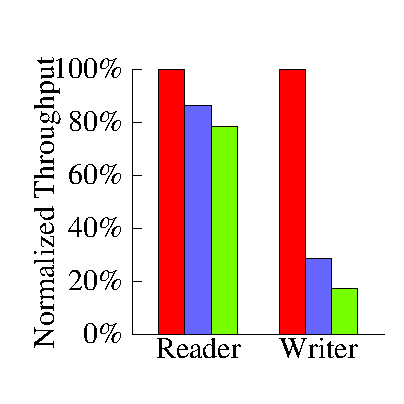
\epsfig{file=iozone.eps,height=100pt}
%\end{multicols}
%\end{figure*}

We evaluated behavioral watchpoints using a microbenchmark and measured the performance of common filesystem operations on an in-memory disk. Our tests ran on a desktop equipped with an Intel\textregistered\ Core\texttrademark\ 2 Duo 2.93 GHz CPU with 4GB physical memory. %Watchpoint instrumentation was enabled for every memory operation. We measured the overhead of the watchpoint framework using a null client and heap-based buffer overflow detector. %We also evaluated the performance of heap-based buffer overflow detector developed using watchpoints.
%we used a null client and a heap-based buffer overflow detector to measure the overhead of using watchpoints. 
%The null client includes the instrumentation for dereferencing watchpoint address.
%To evaluated the cost of watchpoint framework we used a null client 
%and we evaluated the cost of using watchpoint framework with null client and heap-based buffer overflow detector which we developed as one of the application. 
%buffer overflow detecting watchpoints were added to all memory returned from kernel heap allocators.
%We compare native execution, passive execution, and active execution to evaluate the performance of our watchpoint implementation. Passive and active execution both run the Granary DBT framework; however, passive execution only performs basic translation of module code, while active execution translates and adds watchpoint-specific instrumentation to module code. Our choice of network and filesystem modules depend on the fact that they are
%\paragraph{Microbenchmark} %We performed a microbenchmark consisting of a tight-loop of memory operations which exhibits the worst-case overhead of using the watchpoint framework.% with null client and buffer-overflow detector. 
The microbenchmark performed a tight-loop of memory operations and exhibits the worst-case CPU overhead of the baseline watchpoints instrumentation (3.8{\footnotesize$\times$}). For the same microbenchmark, the buffer-overflow detector's overhead was {$\approx$}21{\footnotesize$\times$}, which is caused by the instrumentation needed for precise bounds checking.


%The extra cost of the buffer-overflow detector comes from the instrumentation required for bounds checking.

% We also evaluated the heap-based buffer overflow detector

%The CPU overhead of watchpoint instrumentation was 3.8{\footnotesize$\times$} 



%and we evaluated the buffer-overflow detection application


%using the watchpoint framework with null client was 3.8{\footnotesize$\times$} and buffer-overflow was 21{\footnotesize$\times$}. The extra cost of the buffer-overflow detector comes from the instrumentation required for bounds checking.


%Null client only gives the cost of watchpoint instrumentation.


%performed a tight-loop of memory operations and 


%exhibits the worst-case performance overhead of using watchpoint framework with null client and buffer overflow detector.

 %(about 20{\footnotesize$\times$}). This is expected because our instrumentation adds roughly 13 instructions to each memory load and store. 

%\paragraph{\texttt{rcutorture}} We tested the \texttt{rcutorture} kernel module. It exhibited interesting behavior: all threads experienced a minimum of 6{\footnotesize$\times$} overhead; however, readers were abnormally penalized and tended to see more stale data. We think this is because each writer synchronized with fewer readers.

%\paragraph*{Netperf} We tested network throughput and latency using the \texttt{e1000e} network device driver module. CPU utilization increased by {\texttildelow}6\%, UDP throughput decreased by at most 50\%, TCP throughput was unaffected, and both the TCP and UDP request-response latency increased by no more than 50\%. 

\paragraph{IOzone} The IOzone benchmark creates two processes (one reader and one writer) that perform common file operations on a file of size 480Mb with a record size of 1Kb. 
In our experimental setup, we mounted the \texttt{ext3} filesystem on a 1GB RAMDisk to eliminate the high overhead of disk I/O, which would hide the CPU overhead of adding instrumentation.  We also ensured that all operations go through the file system module code by enabling direct I/O to avoid the effect of the buffer cache.  The mount operation loads two kernel modules: the \texttt{ext3} filesystem module and the \texttt{jbd} journaling module. Watchpoints were added to addresses returned by the two most-used allocators in \texttt{ext3} and \texttt{jbd}: \texttt{\_\_kmalloc} and \texttt{kmem\_cache\_alloc}. 

\Figref{iozone-workload-overhead} shows the drop in throughput of filesystem operations relative to native execution when using Granary and the watchpoints instrumentation.  The \emph{Granary} bar shows the cost of the dynamic binary instrumentation framework on which we build watchpoints.  The \emph{Watch None} bar represents the overhead of baseline watchpoints instrumentation with no added watchpoints. In this configuration, module code has added instrumentation to check each memory access instruction for watched addresses, however, no additional action is needed since no objects are watched.  The \emph{Watch All} bar shows the overhead where all module-allocated objects are watched. In this case, we see two costs.  First, instrumented module code must check for watched addresses and convert them to their unwatched counterparts to perform the memory access. Second, when uninstrumented kernel code accesses a watched address, we must handle the resulting fault and perform some limited instrumentation around the faulting instruction. Finally,  \Figref{iozone-workload-overhead} also shows the overhead of the heap-allocated buffer overflow detector using behavioral watchpoints. This case includes the cost of executing the appropriate watchpoint vtable function to check the bounds on each watched memory access.

The overhead of watching all module-allocated objects is high ({$\approx$}70\%) because many watched objects are accessed by uninstrumented kernel code, which results in many hardware exceptions. Our system recovers from these exceptions by instrumenting kernel code on-demand. We discovered that \texttt{inode}s are frequently accessed by the kernel (thus causing many exceptions) and that not watching \texttt{inode}s improves the performance of \emph{Watch All} to be near that of \emph{Watch None}. We also observed that the added cost of \emph{Buffer Overflow} is smaller than expected, considering the additional work that it performs. This result again suggests that the overhead in \emph{Watch All} is dominated by the cost of faults and our recovery mechanism, thereby masking the cost of the bounds checking.  We are exploring strategies to automatically adapt the granularity of instrumentation to reduce repeated faults in core kernel code.

%The overhead of the watchpoint framework increases to {\texttildelow}70\% when all objects allocated by the module are watched. This is because of the leaked watched objects causing hardware traps in the kernel when dereferenced. We also studied the access pattern of these watched objects and it shows that file system \texttt{inode} objects gets accessed maximum by the kernel and watching them cause maximum number of hardware traps. The overhead of \emph{watch\_all} decreases by {\texttildelow}50\% and become close to the overhead of baseline instrumentation i.e, \emph{watch\_none} after removing watchpoints from \texttt{inode} objects. 

%We also evaluated the selective instrumentation by watching \texttt{inode}, non-\texttt{inode} and only module accessed objects. It reduces the overhead of using the watchpoint framework to {\texttildelow}5\% when only module accessed objects are watched.  
%many of these watched objects are shared and leak to the kernel. When these objects are dereferenced in the kernel, they cause hardware traps because Granary detaches itself at the kernel interface and the watchpoint instrumentation is no longer added to the memory references. These hardware traps are costly and re-attach the watchpoint framework which then instruments the kernel code transitively.
%\Figref{iozone-workload-overhead} also shows the overhead of the heap-allocated buffer overflow detector using behavioral watchpoints. %Our implementation of the buffer-overflow detector does not yet use various optimizations offered by Granary at the instrumentation and wrapper layer, and thus exhibits high overhead.


\begin{figure}[t!]
%\subfloat{
%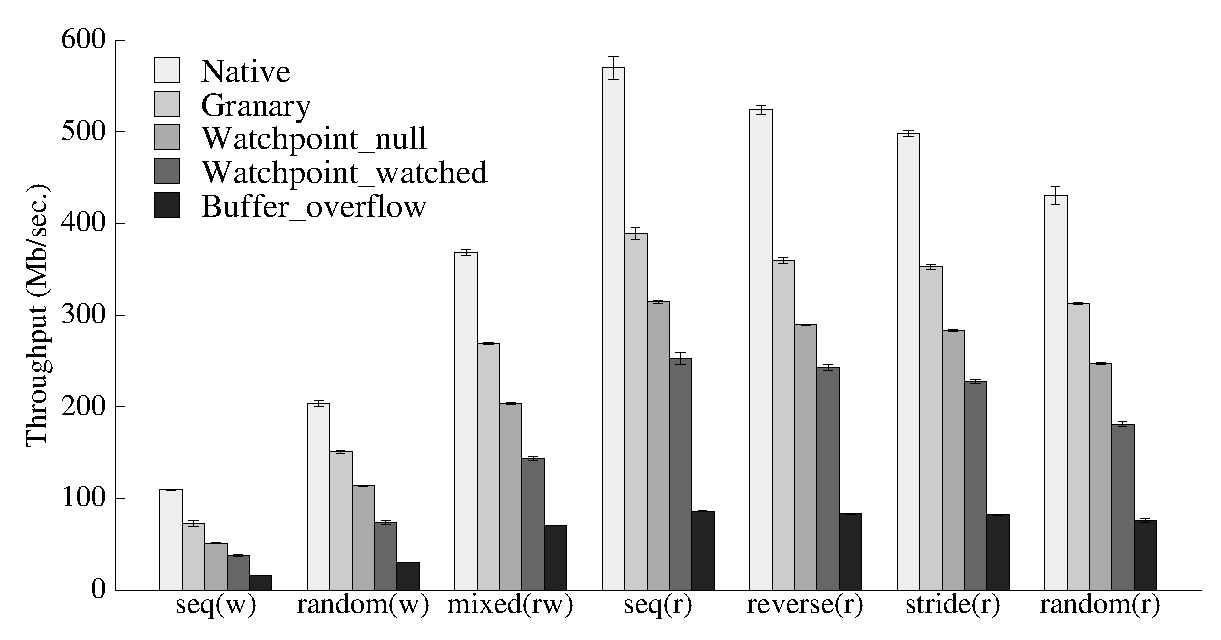
\epsfig{file=watchpoint.eps,width=2.9in, height=1.4in}
%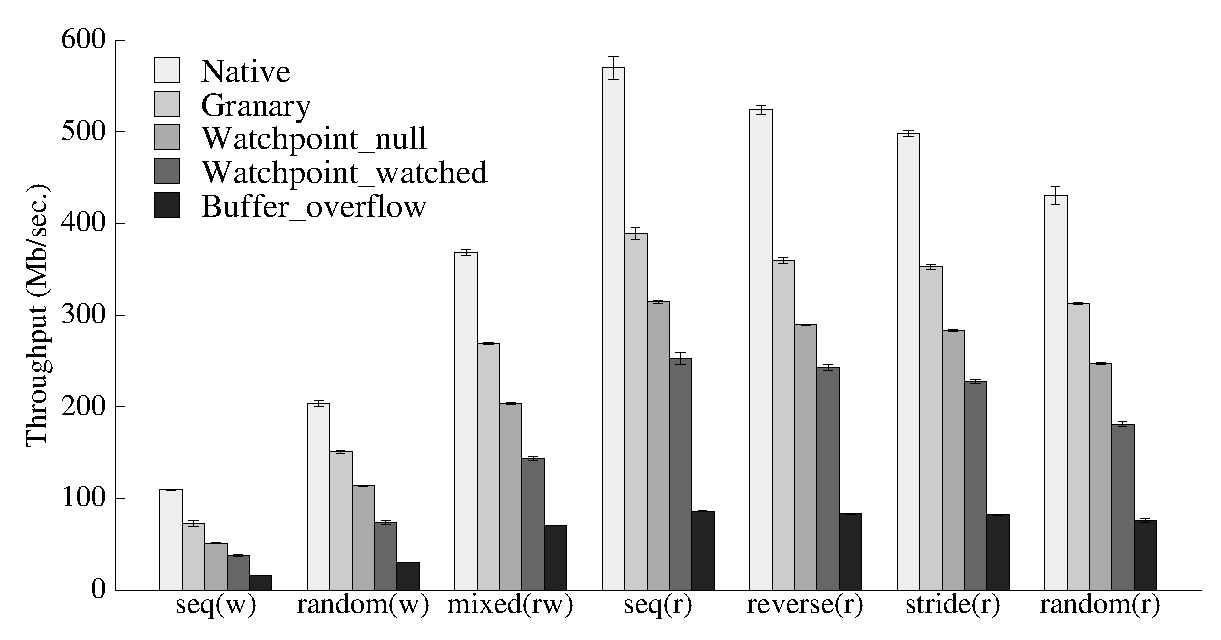
\epsfig{file=watchpoint.eps,width=.99\linewidth}
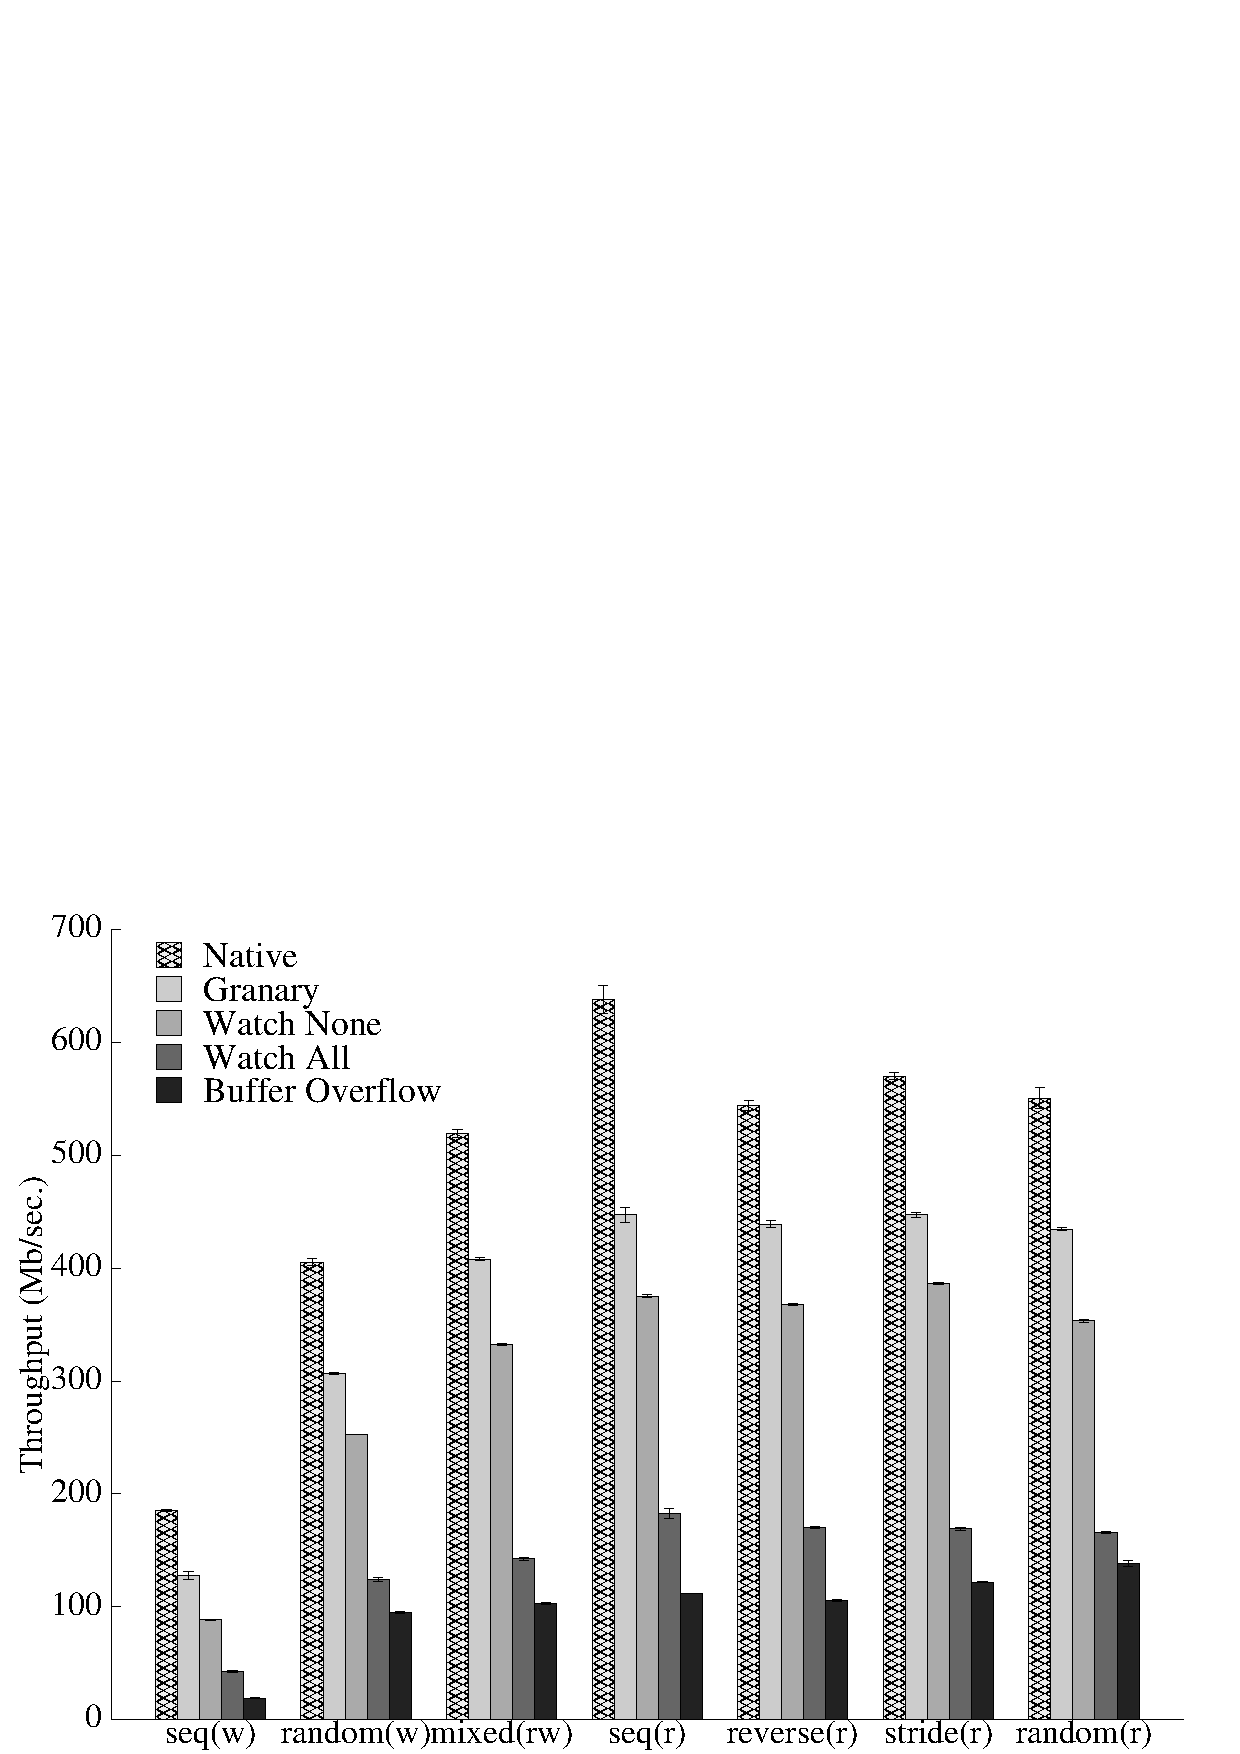
\includegraphics[width=\linewidth]{watchpoint_overflow.pdf}
 %}
%--------sigalternate----------
\vspace{1pt}
\caption{\label{fig:iozone-workload-overhead} Throughput (in Mb/sec) for common file system operations (write workloads (w), read workloads (r)).}
\end{figure}

%overhead of using watchpoints for debugging purpose. 



 %with different clients. \emph{watchpoint\_null} represents the 


%. Watchpoint\_watched shows the  


%using the watchpoint framework leads to a further drop of {\texttildelow}20\%




%We studied the I/O performance of \texttt{ext3} module using IOzone while running it with the watchpoint framework.
%The \texttt{ext3} module was mounted on ramdisk of size 1GB to avoid disk I/O bottleneck and measure the CPU overhead. IOzone creates two reader/ writer processes each operating on a file of 480MB written in 1Kb records. We also enabled the direct I/O to avoid the effect of buffer cache. 
%Watchpoint framework is developed over Granary, a DBT framework. To study the performance overhead of the watchpoint framework, we first evaluated the overhead of Granary by running it with null client. This is the minimum cost associated with any client developed over Granary. We compared the performance of Granary with the watchpoint framework using the null client. The null client doesn't add watchpoints and gives the cost of using watchpoint instrumentation. We also wrapped the two most used allocators of \texttt{ext3} (e.g., \texttt{\_\_kmalloc} and \texttt{kmem\_cache\_alloc}) to add watchpoints to the allocated objects. 
%As shown (\Figref{iozone-workload-overhead}), Granary itself causes a drop in throughput by {\texttildelow}35\% and using the watchpoint framework leads to a further drop of {\texttildelow}20\%. We also noticed that there is a further drop of {\texttildelow}10\% in throughput by adding watchpoints with \texttt{ext3}-allocated object. This is because many of these watched objects were shared with the kernel and any attempt to dereference them triggers the hardware-exception and attaches the watchpoint framework, instrumenting a part of the kernel code. These overheads are acceptable for a tool that detects complex memory usage bugs.



%in kernel environment modules and kernel frequently shares object, thus many of these watched objects gets passed to the kernel. Any attempt to dereference them triggers hardware-exception and attaches watchpoint framework instrumenting part of kernel code. 



%when watchpoint gets added with the  


%We also counted the number of active watchpoints used by \texttt{ext3}.    



%using null client on watchpoint framework.       

%To measure the overhead of watchpoint framework 



%and 


%tested the throughput of disk read and write operations with \texttt{ext3} file system module mounted on a ramdisk of size 1GB. 


%Iozone creates two reader/writer thread in each case and perform the different file operations on a file size of 480MB written in 1Kb records. For evaluation we enabled the direct I/O to remove the effect of buffer cache and perform all operation on disk.


%a file size of 512Kb written in 4Kb records, and with a single reader/writer thread in each case. The throughput for reads and writes decreased by  {\texttildelow}20\% and {\texttildelow}80\%, respectively.

%the throughput of file reads by a single reader thread decreases by , and the throughput of file writes by a single writer thread decreases by {\texttildelow}80\%.
%Our testing environment includes running our system with active (actively looking for watchpoint) and passive (null instrumentation) mode.
%On the microbenchmark, passive instrumentation has a 4\% overhead and active instrumentation has a 20x overhead. For the \texttt{rcutorture} module, 
%the overhead of passive instrumentation is 4\% and the overhead of active instrumentation is 20x
%under a worst-case scenario with a microbenc
%Our evaluation of the performance of behavioral watchpoints 

\section{Related Work}
%Watchpoints are an important debugging facility that help developers track accesses to memory. Most state-of-the-art processors provide some support for hardware watchpoints, but such watchpoints are usually scarce or require specialized hardware support \cite{Mondrix,UnlimitedWatchpoints}. 

%\paragraph{Hardware-based}
Greathouse \emph{et al.}~\cite{UnlimitedWatchpoints} propose a hardware solution that efficiently supports an unlimited number of watchpoints. Witchel and Asanovic \cite{Mondrix} describe the implementation of memory protection domains for the Linux kernel. Protection domains are implemented using specialized hardware and enable fine- and coarse-grained memory protection using a mechanism similar to hardware watchpoints. Unlike our approach, both of these depend on specialized hardware and require that applications using this hardware separately maintain context-specific information. Suh \emph{et al.} \cite{SecureProgramExecFlowTracking} propose a method of secure program execution by tracking dynamic information flow. Memory tagging at the hardware level allows their system to track tainted data as it propagates through a running program. Behavioral watchpoints are similar insofar as a watched address is tagged, and this tag propagates through a program.


%makes the case for supporting an unlimited number of watchpoints. A hardware solution is proposed and multiple applications are described. Unlike our approach, the cited approach depends on specialized hardware and requires that applications using these watchpoints maintain their own context-specific information.

%In , 

%\paragraph{Software-based}
Zhao \emph{et al.} \cite{DynamoRIOWatchpoints} describe a method of implementing an efficient and scalable DBT-based watchpoint system. It uses page protection and indirection through a hash table to track watched memory. This approach supports neither watching ranges of memory, nor context-specific information. Lueck \emph{et al.} \cite{PinADX} introduce semantic watchpoints as part of the PinADX system. %, an extension of the PIN DBT framework. 
It enables interactive debugging by triggering debugger breakpoints when semantic conditions are met. While similar in spirit to behavioral watchpoints, semantic watchpoints do not maintain context-specific, per-watchpoint state. 

%In this respect, a semantic watchpoint is similar to a behavioral watchpoint whose vtable functions trap when a semantic condition is met.
% using DynamoRIO, a popular user-space DBT framework. The method described is very efficient, but unlike behavioral watchpoints, views memory as an opaque sequence of bytes. 
%There have been several proposals on implementing watchpoints in software. 
%Zhao introduced a method for supporting millions of software-based watchpoints using DynamoRIO, a popular user-space DBT framework \cite{DynamoRIOWatchpoints}. Their method is very efficient and does not require inspecting all memory. 
%Our approach differs from theirs in that we e
%Our approach differs from them in the sense that our watchpoint contains the contextual information which can be used for debugging. 
%In , 
% can add a data breakpoint at an address and any access of the gets checked. Unlike this our approach of behavioral watchpoint watches the range of addresses and a watchpoint monitors the access of an object.  Our approach of watchpoint is also viral and any address derived from the watched addresses will also get watched. Our watchpoint implementation bears a resemblance with {cite dynamic information flow} however we donÕt require hardware support to efficiently store the tag else it gets embedded with the address itself.


\section{Conclusions and Future Work}
%We created behavioral watchpoints with the goal of simplifying the implementation of program analysis and debugging tools. We implemented behavioral watchpoints in software because hardware approaches to watchpoints do not meet the needs of program analysis tools. We identified an incongruency between how existing software implements watchpoints and how program analysis tools use watchpoints. Finally, we overcame this incongruency by developing a new form of watchpoint that maintains its own context-specific information---information that is required for large-scale program analysis. We demonstrated the usability of behavioral watchpoints by describing the implementation of three memory error detection and protection policies.

We created behavioral watchpoints to simplify the implementation of DBT-based program analysis and debugging tools. Behavioral watchpoints 
%are a new type of software watchpoint, which 
address both the scalability limits of hardware watchpoints and the lack of contextual information with traditional software watchpoints.  The key innovation is to maintain context-specific information about the memory being watched, which is required for large-scale program analysis, with the watchpoint itself.  Thus, behavioral watchpoints resolve the incongruency between how existing software implements watchpoints and how program analysis tools use watchpoints. We demonstrated the usability of behavioral watchpoints by describing several memory error detection and protection applications. Although our current evaluation is limited, the overheads of behavioral watchpoints
%, as implemented in Granary, 
are quite reasonable for the target use of debugging kernel modules.

As future work, we will investigate the applicability of behavioral watchpoints for isolating and enforcing control-flow integrity policies on Linux kernel modules.


%Behavioral watchpoints make it easier to implement program analysis and 

%overcome the incongruency


%We have established that behavioral watchpoints are useful for implementing memory error detection and protection policies. In summary, we conclude.

% The bibliography should be embedded for final submission.
\bibliographystyle{abbrv}
\bibliography{library}
\end{document}


